\chapter{System Results}
\label{system-results}
Serious development of the RadGrad system began in September 2016. We first created mockups based off the system requirements presented in the System Design section. We then decided on a few key design patterns to follow (i.e. color schemes, layouts, general site organization, etc.). Over the next few months, we continued to change and narrow down our design, until we were able to deploy a working beta version for students, advisors, and alumni. We were then able to test the system with real users, and use the feedback to further improve upon the system. In this chapter, I present the current state of the RadGrad system as of June 2017.

\section{Development}
\subsection{Frameworks and Environments}
RadGrad was built using the Meteor JavaScript web framework. Meteor is integrated with MongoDB and uses the Distributed Data Protocol and publish-subscribe pattern to create real time, responsive code that automatically updates data changes to the client. On the client side, RadGrad uses jQuery and Semantic UI to design and create the user interface. Due to excellent Meteor integration, RadGrad was developed using IntelliJ IDEA. In an effort to create clean and uniform code, RadGrad uses ESLint to confrom to the AirBnB Javascript Style Guide. 

\subsection{Project Management}
We developed RadGrad using GitHub issues and GitHub projects. Development tasks are created as a GitHub issue, and each issue has an assigned developer and and assigned branch. Each issue also resides in a GitHub project, which groups issues together to mark larger milestones. When the developer begins actively working on the issue, they will move the issue in the milestone from a ``Backlog" column to an ``In Progress" column. Once the developer completes the task in the specified branch, they will close the issue and move the issues in the milestone from the ``In Progress" column to the ``Done" column. The RadGrad developers typically communicate through Slack and in person meetings twice a week. 

\section{Data Model}
\subsection{Career Goals}
\begin{figure}[htbp!]
\centering
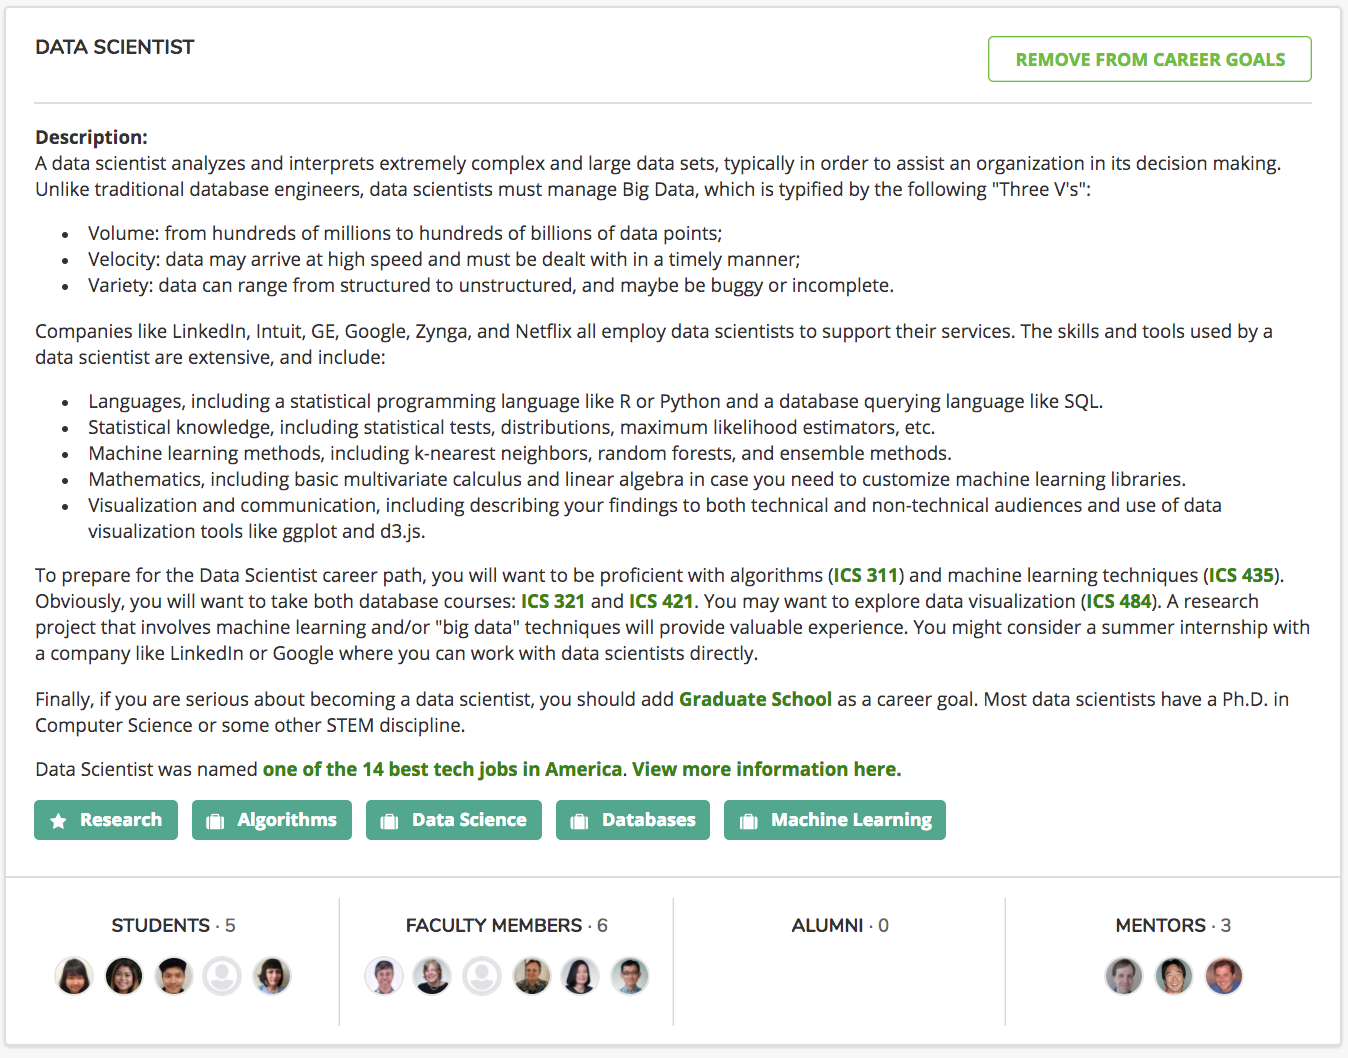
\includegraphics[width=1.0\textwidth]{dm-career}
\caption{Example of a career goal representation.}
\end{figure}
Career goals represent possible ICS related careers that ICS students can aspire to get after graduation (Figure 6.1). Each career goal has an associated name, slug, description, related interests, and an optional URL for more information. Students can choose as many career goals as they want. Faculty and mentors can choose career goals that they would like to be associated with as well. Possible career goals as of June 2017 are listed in Table 6.1.

\begin{table}[htbp!]
\centering
\begin{tabular}{ l l l } 
 Data Scientist & Database Administrator & DevOps Engineer \\ 
 Full Stack Developer & Game Developer & Graduate School \\ 
 Information Security Analyst & Information System Manager & IoT Architect \\ 
 Mobile App Developer & Network Engineer & Research Scientist \\
 Robotics Engineer & Software Developer & Startup Co-Founder \\
 Teacher & UX Designer & VR/AR Engineer 
\end{tabular}
\caption{List of RadGrad career goals as of June 2017}
\label{table:1}
\end{table}

\subsection{Courses}
\begin{figure}[htbp!]
\centering
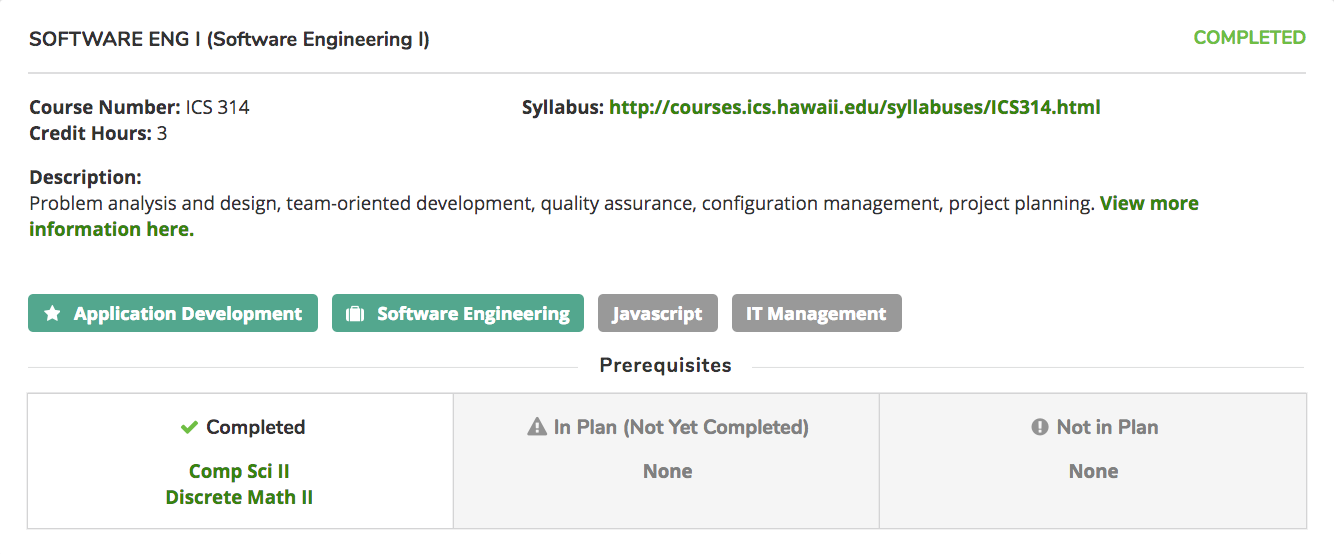
\includegraphics[width=1.0\textwidth]{dm-course}
\caption{Example of a course representation.}
\end{figure}
Courses represent all past, present, and future ICS courses (Figure 6.2). Each course has an associated name, short name, slug, course number, description, credit hours, related interests, a syllabus URL, a URL for more information, and associated prerequisites. The course name is the official name appearing in the UH registration guide, and the course short name is used for display purposes. Students may add as many courses as they would like to their degree plan. 

Course instances represent individual instances for each student. Each course instance has an associated semester, course, whether it has been verified or not, whether it came from STAR or not, grade, credit hours, note, student, and associated ICE points. A past course instance is always considered verified if it is from STAR. Course instances from STAR from the current or future semesters are not considered verified yet since there is no official grade. Special courses that are manually input (not from STAR) could also be considered verified by an advisor. A course instance has a note if it is not an ICS course. It is important to note that course instances on RadGrad are only valid on RadGrad, and students must use other methods to officially make UH course registration changes.

\subsection{Desired Degrees}
\begin{figure}[htbp!]
\centering
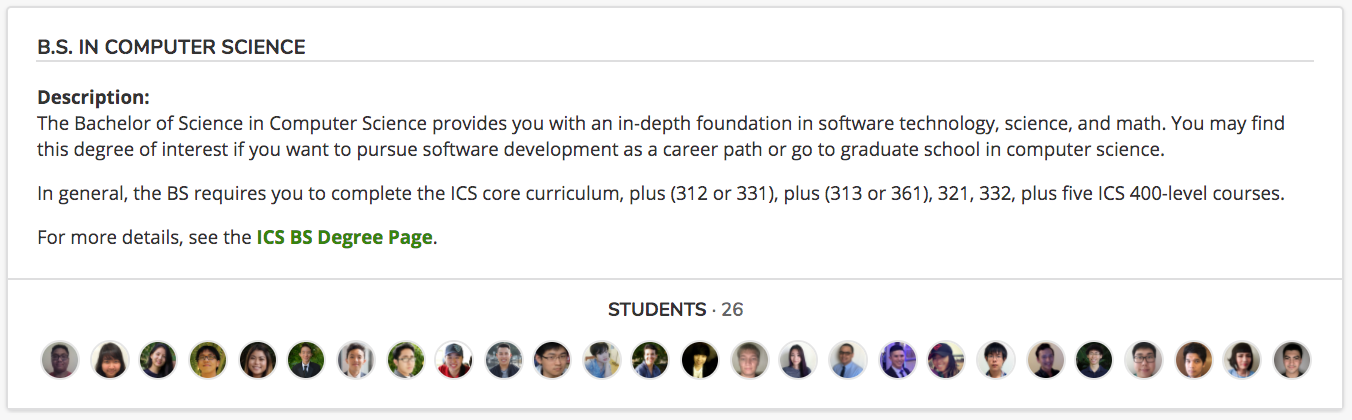
\includegraphics[width=1.0\textwidth]{dm-degree}
\caption{Example of a desired degree representation.}
\end{figure}
Desired degrees represent all past, present, and future ICS degrees (Figure 6.3). Each desired degree has an associated name, short name, slug, and description. Students can only choose one desired degree at any given time. However, they are free to switch desired degrees as many times as they want. It is important to note that desired degrees on RadGrad are only valid on RadGrad, and students must use other methods to officially change their declared degree at UH. 

\subsection{Degree Plan}
\begin{figure}[htbp!]
\centering
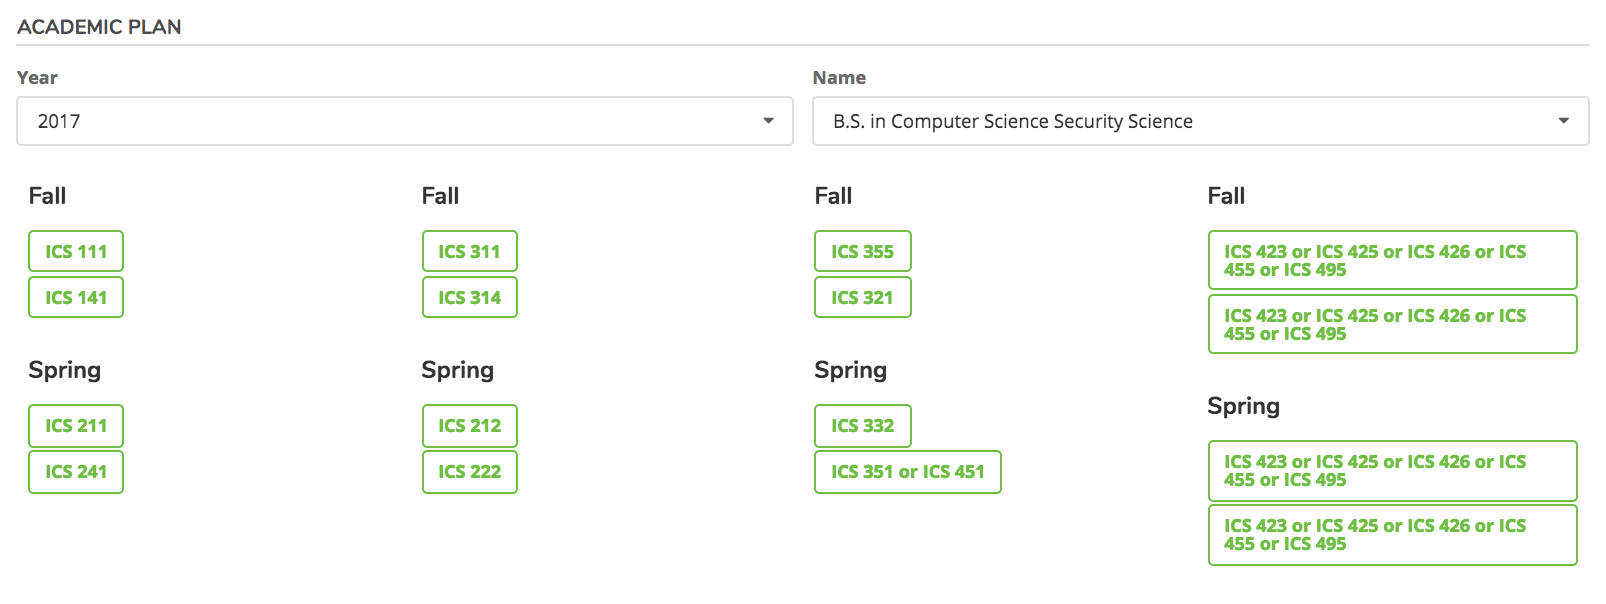
\includegraphics[width=1.0\textwidth]{dm-degreeplan}
\caption{Example of a degree plan representation.}
\end{figure}
Degrees plans represent all past, present, and future ICS degree plans (Figure 6.4). Each degree plan has an associated degree, name, effective semester, amount of courses per semester, and list of courses. Students can view degree plans if they would like a more specific focus than just a broad BS or BA degree. Examples of degree plans are ``BS in Computer Sciences Security Sciences", ``BA in ICS Security Science Focus", and ``BA in Computer Sciences IT Focus." Students can look at any plan at any time to see what they would need to do to fulfill it. It is important to note that these degree plans change over time, and a ``BS in Computer Sciences Security Sciences" may be different in 2016 than in 2018. This is why both year and plan name must be chosen when selecting a plan.  Degree plans were created to help students to become more aware of and make sense of the different degree plans that they can choose from. Having these representations on RadGrad help students to see how different degree plans would work with their specific interests, career goals, courses, and opportunities. Overall, d
egree plans can help students to narrow down their interests into a more specific field. 

\subsection{Feeds}
\begin{figure}[htbp!]
\centering
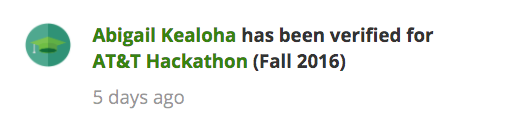
\includegraphics[width=0.5\textwidth]{dm-feed}
\caption{Example of a feed representation.}
\end{figure}
Feeds represent select actions of RadGrad users (Figure 6.5). Each feed has associated users, opportunity, course, semester, description, time stamp of the action, picture, and feed type. A feed could have one or multiple users. There are currently six different feed types: a new RadGrad user is added, a new course is added to RadGrad, a new opportunity is added to RadGrad, a user has been verified for completing an opportunity, a new course review has been added, and a new opportunity review has been added. These particular actions have been selected because they could be useful and of interest to other RadGrad users.

\subsection{Feedbacks}
\begin{figure}[htbp!]
\centering
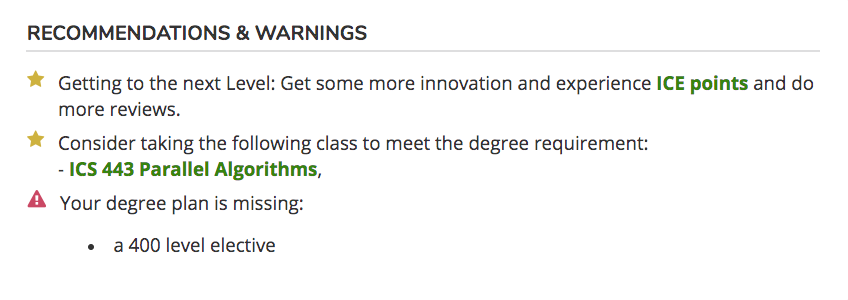
\includegraphics[width=1.0\textwidth]{dm-feedback}
\caption{Example of feedback representations.}
\end{figure}
Feedbacks represent recommendations and warnings for students (Figure 6.6). Each feedback has an associated name, slug, description, and feedback type. There are currently two feedback types: recommendation and warning. 

Feedback instances represent individual instances for each student. Each feedback instance has an associated feedback, user, description, and area. There are currently four different areas: interests, ICE, STAR, and degree plan. Each time the student's plan changes, feedback instances in these areas are deleted and recalculated.

\subsection{Help Messages}
\begin{figure}[htbp!]
\centering
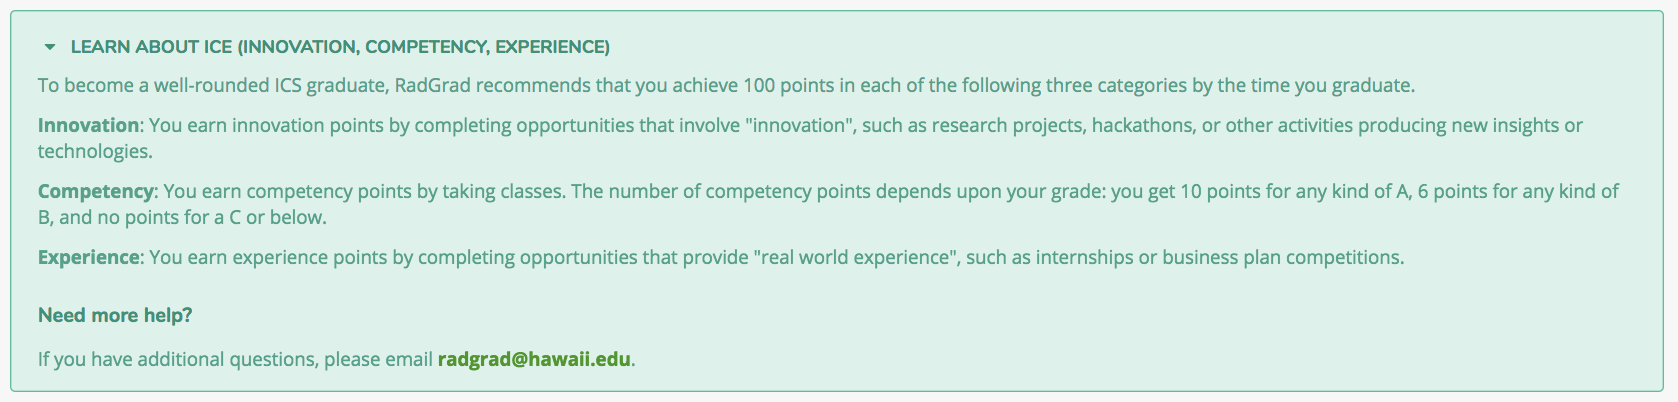
\includegraphics[width=1.0\textwidth]{dm-help}
\caption{Example of a help representation.}
\end{figure}
Help messages represent guidance for a particular RadGrad page (Figure 6.7). Each help message has an associated route name, title, and text. The text can contain actual text, images, and formatting. Each page (route name) can have at most one help message. These help messages are displayed at the top of the specified page, in a collapsible pane.  

\subsection{ICE}
\begin{figure}[htbp!]
\centering
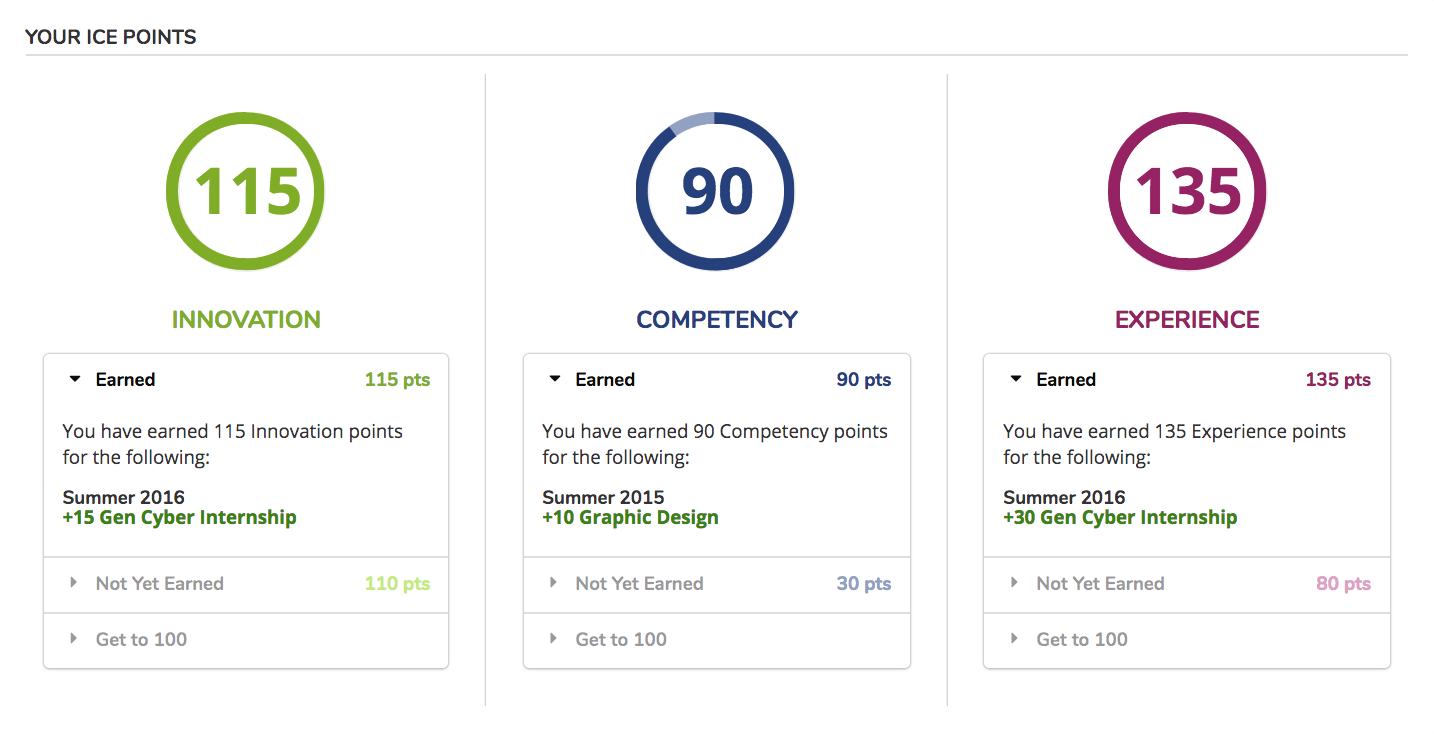
\includegraphics[width=1.0\textwidth]{dm-ice}
\caption{Example of an ICE representation.}
\end{figure}
ICE represents a student's ICE points (Figure 6.8). Each ICE has an associated number for ``I", ``C", and ``E." There are two types of ICE points: earned and planned. Earned ``I" and ``E" points are calculated by adding the ``I" or ``E" points for each verified opportunity in the student's plan. Earned ``C" points are calculated by adding the ``C" points for each verified course in the student's plan. The amount of earned points for each course depends on the grade that the student received; A's represent more points than B's. Planned ``I" and ``E" points are calculated by adding the ``I" or ``E" points for each unverified opportunity in the student's plan. Planned ``C" points are calculated by adding the ``C" points for each unverified course in the student's plan. A student's earned and planned ICE points are updated each time there are changes to the student's degree plan. 

\subsection{Interests}
\begin{figure}[htbp!]
\centering
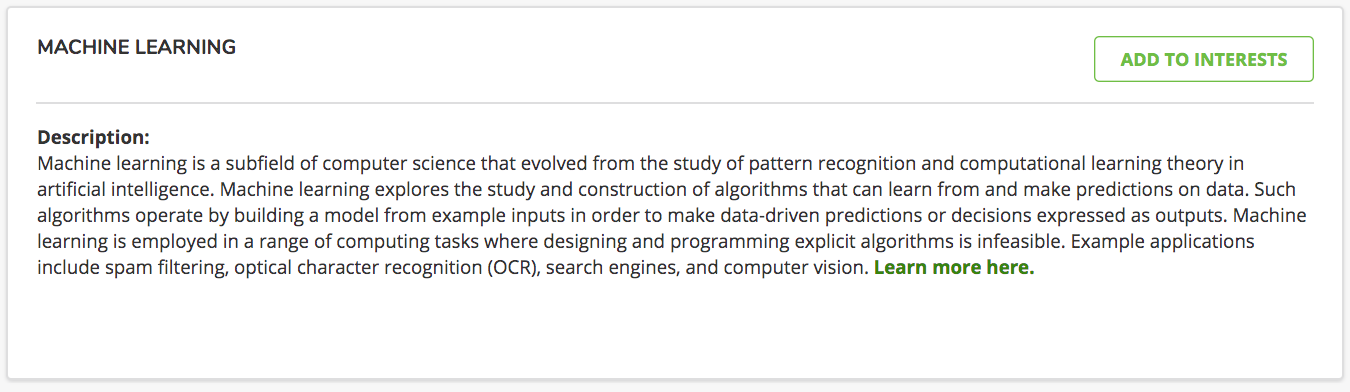
\includegraphics[width=1.0\textwidth]{dm-interests}
\caption{Example of an interest representation.}
\end{figure}
Interests represent possible ICS related interests that RadGrad users could have (Figure 6.9). Each interest has an associated name, slug, description, interest type, and a URL for more information. All RadGrad users may choose to be associated with as many interests as they would like. All current interests on RadGrad as of June 2017 are listed in Table 6.9.

\begin{table}[htbp!]
\centering
\begin{tabular}{ l l l } 
.NET & Algorithms & Android \\ 
Application Development & Artificial Intelligence & Assembler \\
Bioinformatics & Biology & C and C++ \\
C\# & Civic Engagement & Cognitive Science \\
Computer Architecture & Computer Ethics & Computer Graphics \\
Computer Vision & Cryptography & Data Science \\
Data Visualization & Databases & Entrepreneurship \\
Game Design & Graphic Design & Hardware \\
High Performance Computing & Human-Computer Interaction & IT Management \\
Java & Javascript & Linux \\
Lisp & Machine Learning & Mobile Computing \\
Networks & Operating Systems & Parallel Programming \\
Perl & Prolog & Psychology \\
Python & R & Research \\
Robotics & Ruby & Software Development \\
SQL & Security & Sustainability \\
Teaching & Theory of Computation & Unity \\
Virtual Reality & Web Development & iOS
\end{tabular}
\caption{List of RadGrad interests as of June 2017}
\label{table:2}
\end{table}

\subsection{Levels}
\begin{figure}[htbp!]
\centering
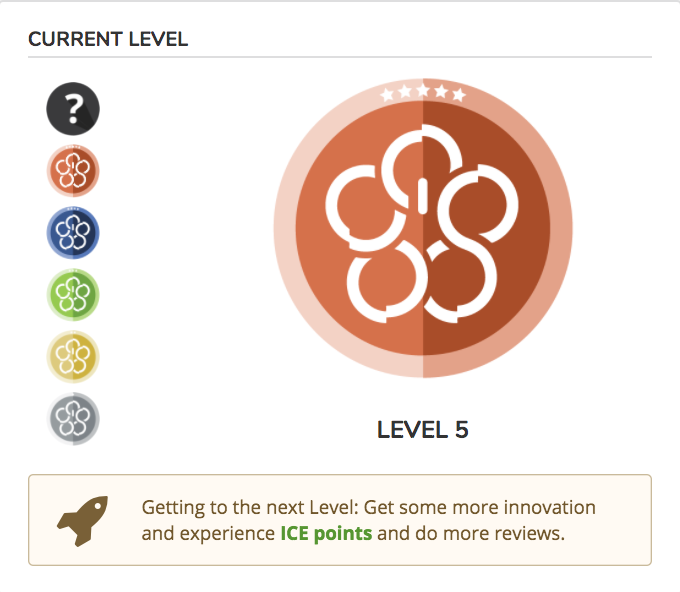
\includegraphics[width=0.5\textwidth]{dm-level}
\caption{Example of a level representation.}
\end{figure}
Levels represent a student's RadGrad level (Figure 6.10). There are six possible levels, from Level 1 to Level 6. A student's level is calculated based off the amount of ICS courses they have passed, the amount of opportunities they have done, and the amount of reviews they have contributed on RadGrad. Levels can be recalculated for all users at any time through the administrator pages.

\subsection{Advisor Logs}
\begin{figure}[htbp!]
\centering

\includegraphics[width=1.0\textwidth]{dm-log}
\caption{Example of an advisor log representation.}
\end{figure}
Advisor logs represent an interaction between an ICS advisor and a student (Figure 6.11). Each advisor log has an associated student, advisor, text, and date created. A new log can be created by the advisor whenever they have a meeting with a student. Advisors and students can use these logs to keep track of when meetings were held, and what occurred at these meetings. 

\subsection{Mentors}
\begin{figure}[htbp!]
\centering
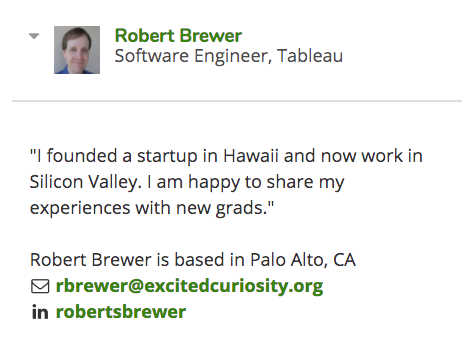
\includegraphics[width=0.5\textwidth]{dm-mentor}
\caption{Example of a mentor representation.}
\end{figure}
The mentor data model includes three parts: mentor profiles, mentor questions, and mentor answers (Figure 6.12). Each mentor profile has an associated mentor, company, career, location, LinkedIn, and a message about what motivated them to become a mentor. Each mentor will have exactly one mentor profile.  

Each mentor question has an associated title, slug, student, whether it is moderated or not, whether it is visible or not, and moderator comments. Students can create as many mentor questions as they would like. However, each question needs to be approved by moderation in order to be visible to the public. Advisors and administrators have the ability to moderate questions. If a question is declined by moderation, the moderator can add reasons for the decline in the moderator comments field. The student can then see the feedback, and they are able to either edit their question and send it back to moderation, or simply discard the question. There is no limit to how long the back and forth process between student and moderator can go on. 

Each mentor answer has an associated question, mentor, and text. Each mentor question can have any amount of mentor answers, but each mentor answer can answer at most one mentor question. Each mentor question can only be associated with exactly one mentor. There is no moderation process for mentor answers, and submitted mentor answers are automatically visible on RadGrad. 

\subsection{Opportunities}
\begin{figure}[htbp!]
\centering
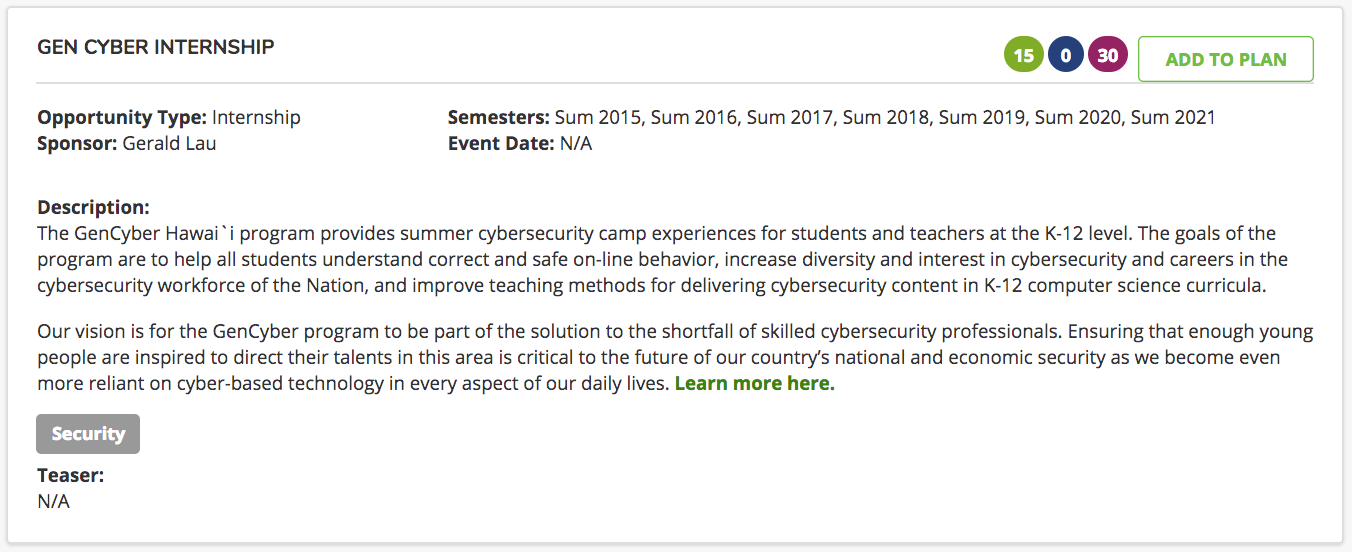
\includegraphics[width=1.0\textwidth]{dm-opportunity}
\caption{Example of an opportunity representation.}
\end{figure}
Opportunities represent all past, present, and future ICS related opportunities (Figure 6.13).  Each opportunity has an associated name, slug, description, opportunity type, sponsor, related interests, icon, semesters available, event date, whether it is an independent study or not, URL for more information, and ICE points. Currently, there are five opportunity types: club, event, internship, online learning, and project. The opportunity sponsor is any faculty member who is the point of contact for the opportunity. If the opportunity occurs on a semester basis, it will have associated semesters. If the opportunity occurs on a specific date, it will have an associated event date. The amount of ICE points varies depending on the nature of the opportunity, and is determined by RadGrad administrators. 

Opportunity instances represent individual instances for each student. Each opportunity instance has an associated semester, opportunity, whether it is verified or not, student, and ICE points. An opportunity instance can only be verified by a RadGrad advisor or faculty. Two students that each have an opportunity instance for the same opportunity could have different ICE points depending on the extent of their involvement in the opportunity.    

\subsection{Public Stats}
\begin{figure}[htbp!]
\centering
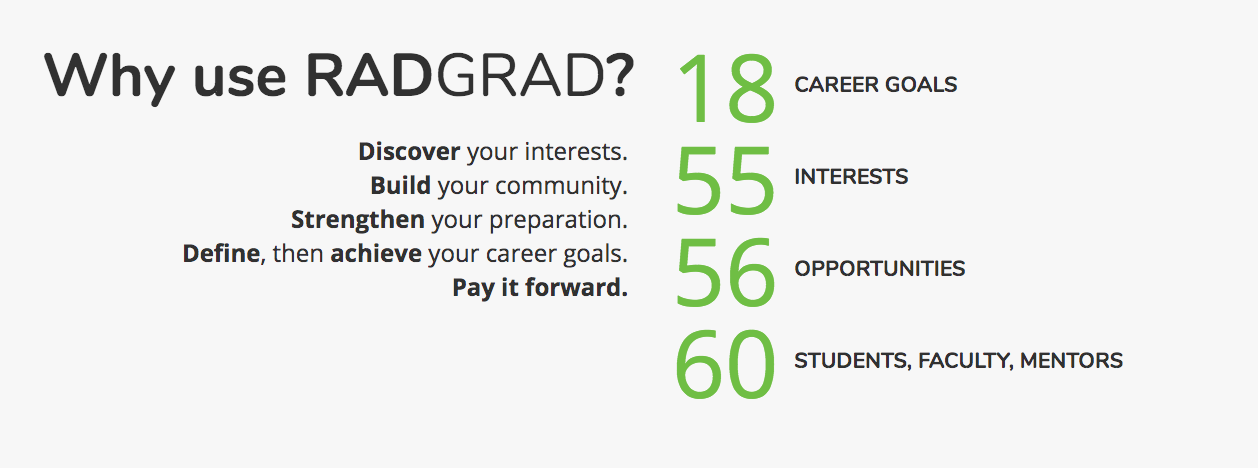
\includegraphics[width=1.0\textwidth]{dm-stats}
\caption{Example of a public stats usage on the landing page.}
\end{figure}
Public stats calculate 24 different RadGrad statistics from the current database (Figure 6.14). The statistics calculated are: total courses, total career goals, list of career goals, total desired degrees, list of desired degrees, total interests, list of interests, total opportunities, total project opportunities, list of project opportunities, total users, total students, total faculty, total mentors, list of mentor professions, list of mentor locations, total course reviews, list of courses reviewed, total level one students, total level two students, total level three students, total level four students, total level five students, and total level six students. Public stats are automatically recalculated once each day at midnight. 

\subsection{Reviews}
\begin{figure}[htbp!]
\centering
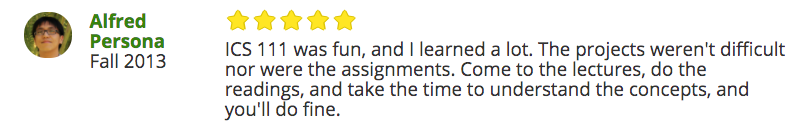
\includegraphics[width=1.0\textwidth]{dm-review}
\caption{Example of a review representation.}
\end{figure}
Reviews represent all course and opportunity reviews written by students on RadGrad (Figure 6.15). Each review has an associated slug, student, review type, reviewee, semester, rating (Figure 6.1), comments, whether it is moderated or not, whether it is visible or not, and moderator comments. There are two review types: course and opportunity. The reviewee refers to the course or opportunity that is being reviewed. Each review must have a rating from one to five stars (Figure 6.16). Each student may review a course once the semester they have taken it in has passed. Each student may review an opportunity once the opportunity has been verified. Each student can review each course or opportunity at most once. Each review is visible to the public by default, but can be removed by moderators. Advisors and administrators have the ability to moderate reviews. If a review is declined by moderation, the moderator can add reasons for the decline in the moderator comments field. The student can then see the feedback, and they are able to either edit their review and send it back to moderation, or simply discard the review. There is no limit to how long the back and forth process between student and moderator can go on. A student can also update their review at any time, but this will mean that the review will go through the moderation process again.

\begin{figure}[htbp!]
\centering
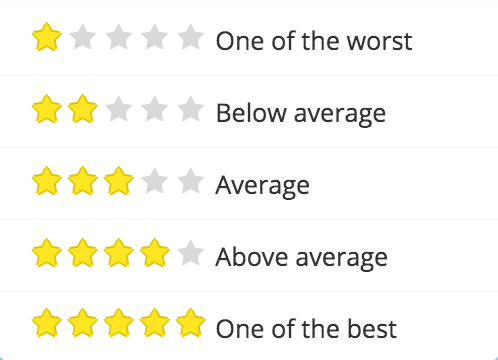
\includegraphics[width=0.3\textwidth]{datamodel-reviews}
\caption{Course and opportunity review ratings.}
\end{figure}

\subsection{Roles}
Roles represent the different user roles allowed in RadGrad. There are currently six roles: faculty, student, admin, alumni, advisor, and mentor. Currently, users are allowed to have exactly one role. All users except for admin and advisor can view only their own RadGrad pages. Advisors can also view student RadGrad pages, and admin can view all RadGrad pages. 

\subsection{Semesters}
Semesters represent an academic semester at the University of Hawaii. Each semester has an associated term, year, number to sort by, semester number, and slug. There are three possible terms: Spring, Summer, and Fall. The number to sort by easily allows chronological comparisons between semesters. Semester number is another number used for sorting semesters, using 2010 as the earliest year. 

\subsection{Slugs}
Slugs are strings used as part of a URL to uniquely identify an entity. These strings do not change with different instantiations of the database like docIDs do. Slugs are used in the RadGrad data model to represent relationships between different entities. Therefore, only collections that need to be referenced by other collections contain a slug. 

\subsection{Teasers}
\begin{figure}[htbp!]
\centering
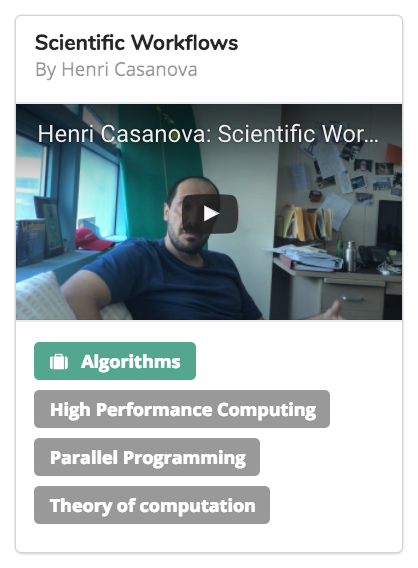
\includegraphics[width=0.5\textwidth]{dm-teaser}
\caption{Example of a teaser representation.}
\end{figure}
Teasers represent short videos that advertise an ICS opportunity (Figure 6.17). Each teaser has an associated title, slug, author, URL, description, duration, related interests, and opportunity. Any member of RadGrad can be an author of a teaser. Teasers are typically less than a minute long and function as a sort of quick advertisement to get potential students interested in participating in that particular opportunity. 

\subsection{Users}
\begin{figure}[htbp!]
\centering
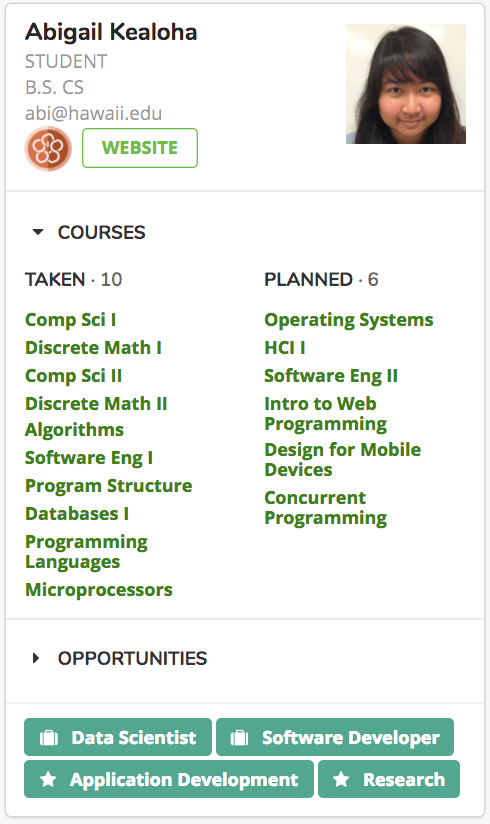
\includegraphics[width=0.5\textwidth]{dm-user}
\caption{Example of user representations.}
\end{figure}
Users represent anyone who has created an account on the RadGrad system (Figure 6.18). Each user has an associated username, first name, last name, slug, email, password, UH ID, career goals, interests, desired degree, picture, level, website, hidden courses, and hidden opportunities. The user's RadGrad username is the same as their UH email name. This, along with their email, cannot be changed once the user's account is created. Only student users will have a desired degree and a level. Hidden courses and hidden opportunities are used to keep track of courses and opportunities that students have actively ``hidden" from their page. By keeping track of these hidden courses and opportunities, students can have the option to make them visible again.

\subsection{Verification Requests}
\begin{figure}[htbp!]
\centering

\includegraphics[width=1.0\textwidth]{dm-verification}
\caption{Example of a verification request representation.}
\end{figure}
Verification requests represent a request from a student to get verification and ICE points for completing an opportunity (Figure 6.19). Each opportunity has an associated date, status, verifier, and feedback. There are three possible statuses: accepted, rejected, and open. The verifier is the user who has verified the event. Only advisors, faculty, and admin can be a verifier. If a request is rejected, the verifier can add reasons for the rejection in the feedback field. The student can then see the feedback and the results of the verification. If the verifier wishes to reopen the verification request, they may do so at any time. A student who would like to reopen a request will need to contact the verifier.  

\subsection{Academic Years}
Academic years represent an academic year at the University of Hawaii. Each academic year has an associated year, spring year, student, and semesters. Since academic years start in the Fall and end in the Summer, they span two years: year, and spring year. A student on RadGrad must have an academic year for each year, or portion of a year, that they are enrolled in an ICS course or participated in an ICS opportunity.

\section{Testing}
\subsection{Interactive Testing}
RadGrad uses interactive server-side testing with Mocha test runner and Chai Expect Assertions during code production in order to maintain correctness. Each collection class from the data model has tests in a corresponding testing file. These tests include checking if a new collection entity can be defined, if a collection entity can be removed, if a collection entity can be dumped from the database, and if a collection entity can be restored from a dump file to the database. If the collection class includes additional functions specific to that collection, the test file includes tests for those functions as well.

\subsection{Personas}
In order to ensure that a wide variety of students will be able to use RadGrad effectively, we created five personas, where each persona is represented with a student user account on RadGrad. Each persona represents a student at a different part of the degree program. Below are brief descriptions of each persona. 

\begin{enumerate}
  \item Ella Zwick: Ella is a Freshman who has just declared her BA ICS major. She has not taken any ICS courses yet, and she does not have a RadGrad degree plan yet either. She is at Level 1. Her career goal is to be a web developer, and her interests are in civic engagement and web development. 
  \item Charley Sherry: Charley is a Freshman who is in his second semester of the BS CS curriculum. He is currently enrolled in ICS211 and ICS241. He is at Level 2. His career goal is to be a data scientist, and his interest is in bioinformatics.  He has at least 12 competency points for completing ICS111 and ICS141 during the previous semester. 
  \item Betty Keanu: Betty is a Junior who has completed the BS CS core curriculum (ICS111, ICS141, ICS211, ICS241, ICS311, ICS314) and is currently taking 300+ courses to fulfill the rest of her degree plan. She is at Level 4. Her career goals are graduate school and data scientist, and her interests are big data, visualization, and research. She has completed a few opportunities, and has at least 30 innovation points, at least 36 competency points, and at least 30 experience points. 
  \item Abigail Kealoha: Abigail is a Junior who is two semesters away from graduating with her BS in CS. She is Level 5. Her career goal is to be a web developer, and her interests are security and software engineering. She has completed several opportunities, and has at least 80 innovation points, at least 80 competency points, and at least 80 experience points. Abigail has also contributed one course review on RadGrad. 
  \item Alfred Persona: Alfred is a Senior in his last semester of the BS CS curriculum. He is at Level 6. His career goal is a software developer and his interests are in game design, hardware, and virtual reality. He has completed many opportunities, and has at least 100 points for each of the ICE categories. Alfred also contributed 6 course reviews on RadGrad.
\end{enumerate} 

\subsection{Beta Testing}
In Spring 2017, after completion of the major Student, Advisor, and Administrator components and pages, we held RadGrad beta tests, which invited selected students and an advisor to view and use the system for the first time. The main goals of these tests were to identify user problems, identify common aspects users like, assess if parts of the user interface are more intuitive or more difficult to use, if there are missing features that should be implemented, if certain features could be improved, and to get a feel of whether users feel that the would use RadGrad and that it would improve their engagement in the ICS degree program. We hoped this data would help us decide if the system so far is going in a promising direction.

\subsubsection{Student Beta Testing}
Student subjects were solicited over email, and were selected in a way that provided us with a wide range of student levels. Each student was given \$20 as compensation for 30 minutes of their time. Prior to the testing session, each subject provided their name and UH account, completed ICS courses, completed opportunities, interests, and career goals. Using this information, the student's RadGrad account was set up prior to the session. Each session involved one student and two RadGrad developers (an evaluator to lead the session, and an observer). At the start of the session, the evaulator briefly went over the basic ideas of the system and the different parts that they can interact with. During the second part of the session, the student was allowed to peruse the system and explore or comment on anything they found particularly interesting. During the third part of the session, the evaluator asked the student to describe what they liked about the system, what they disliked about the system, and whether or not they think they would use this system if it were available to them. See Table 6.3.

\begin{table}[htbp!]
\centering
\begin{tabular}{ |p{8cm}|p{8cm}|}
 \hline
\textbf{Positive Feedback} & \textbf{Problems with System} \\
 \hline
 Recommended opportunities are useful because otherwise students are only notified by Gerald's emails  & ICE points display was confusing \\
 \hline
 Reduces the amount of work currently needed for students who try to find ways to succeed beyond the classroom. &List of opportunities was hard to view because it was partially off the screen\\
 \hline
 Degree planner helpful for visualizing pathway &Annoying to have to scroll to see all possible review ratings\\
  \hline
Likes the levels and ICE gamification &Confusing to find some things without some kind of tutorial \\
 \hline
Level stickers can help students see who they might want to talk to &Performance issue with page loading times \\
 \hline
RadGrad and ICE are good at stressing the importance of activities outside of courses &Wish there were notifications for when new opportunities come up\\
 \hline
RadGrad provides extra details about courses and opportunities that were previously unknown to the student &Recommended Courses and Recommended Opportunity widgets on the student home page have non-intuitive scrolling behavior\\
 \hline
RadGrad helps degree plan to feel less ``random" &Wish there were notifications for when new opportunities come up\\
 \hline
Likes how RadGrad helps students understand the benefits of internships, which they learned too late would be helpful &Students should be allowed to opt out of showing their current and future courses and opportunities\\
 \hline
RadGrad is a good way to keep track of a degree plan, which a student previously wrote on a paper and misplaced it & Wish there were notifications for when new opportunities come up \\
 \hline
 STAR does not work adequately for many students, and RadGrad could be a good supplement for that & Wish there was less unnecessary clicking while altering the degree planner\\
 \hline
Student easily navigated degree planner UI with only some guidance &Wish there were support for specific focus areas\\
 \hline
Mentorspace could help students to get an idea of what they can actually do with their degree after graduation &Would like to know ahead of time when certain courses are being offered\\
 \hline
The fact that RadGrad helps you plan even if you have no idea what you want to do, whereas with STAR, you have to know what you want to do beforehand & Manual edits to one student's generated plan caused empty extraneous years in the degree planner\\
 \hline
Rating courses seems helpful in planning & One student's STAR data included a long gap between years, which wasn't handled well in the degree planner without manual intervention\\
 \hline
Liked how degree plan could be generated rather than manual &\\
 \hline
Liked the idea of an individual ICS online space &\\
 \hline
\end{tabular}
\caption{Student beta test results}
\label{table:3}
\end{table}

\subsubsection{Advisor Beta Test}
It was easier to solicit an advisor for the beta test, since Gerald Lau is currently the only ICS advisor. During his session, the evaluator briefly went over the system from the point of view of both students and the advisor. While Gerald did not actually get to interact with the system himself, he was able to see how it would be used, and he was able to give feedback about his perceived usefulness of the system. Gerald's response was positive overall, and he seemed interested in integrating it into future advising.
\section{Student Mode}
\subsection{Degree Planner}
\subsubsection{Degree Planner}
\begin{figure}[htbp!]
\centering
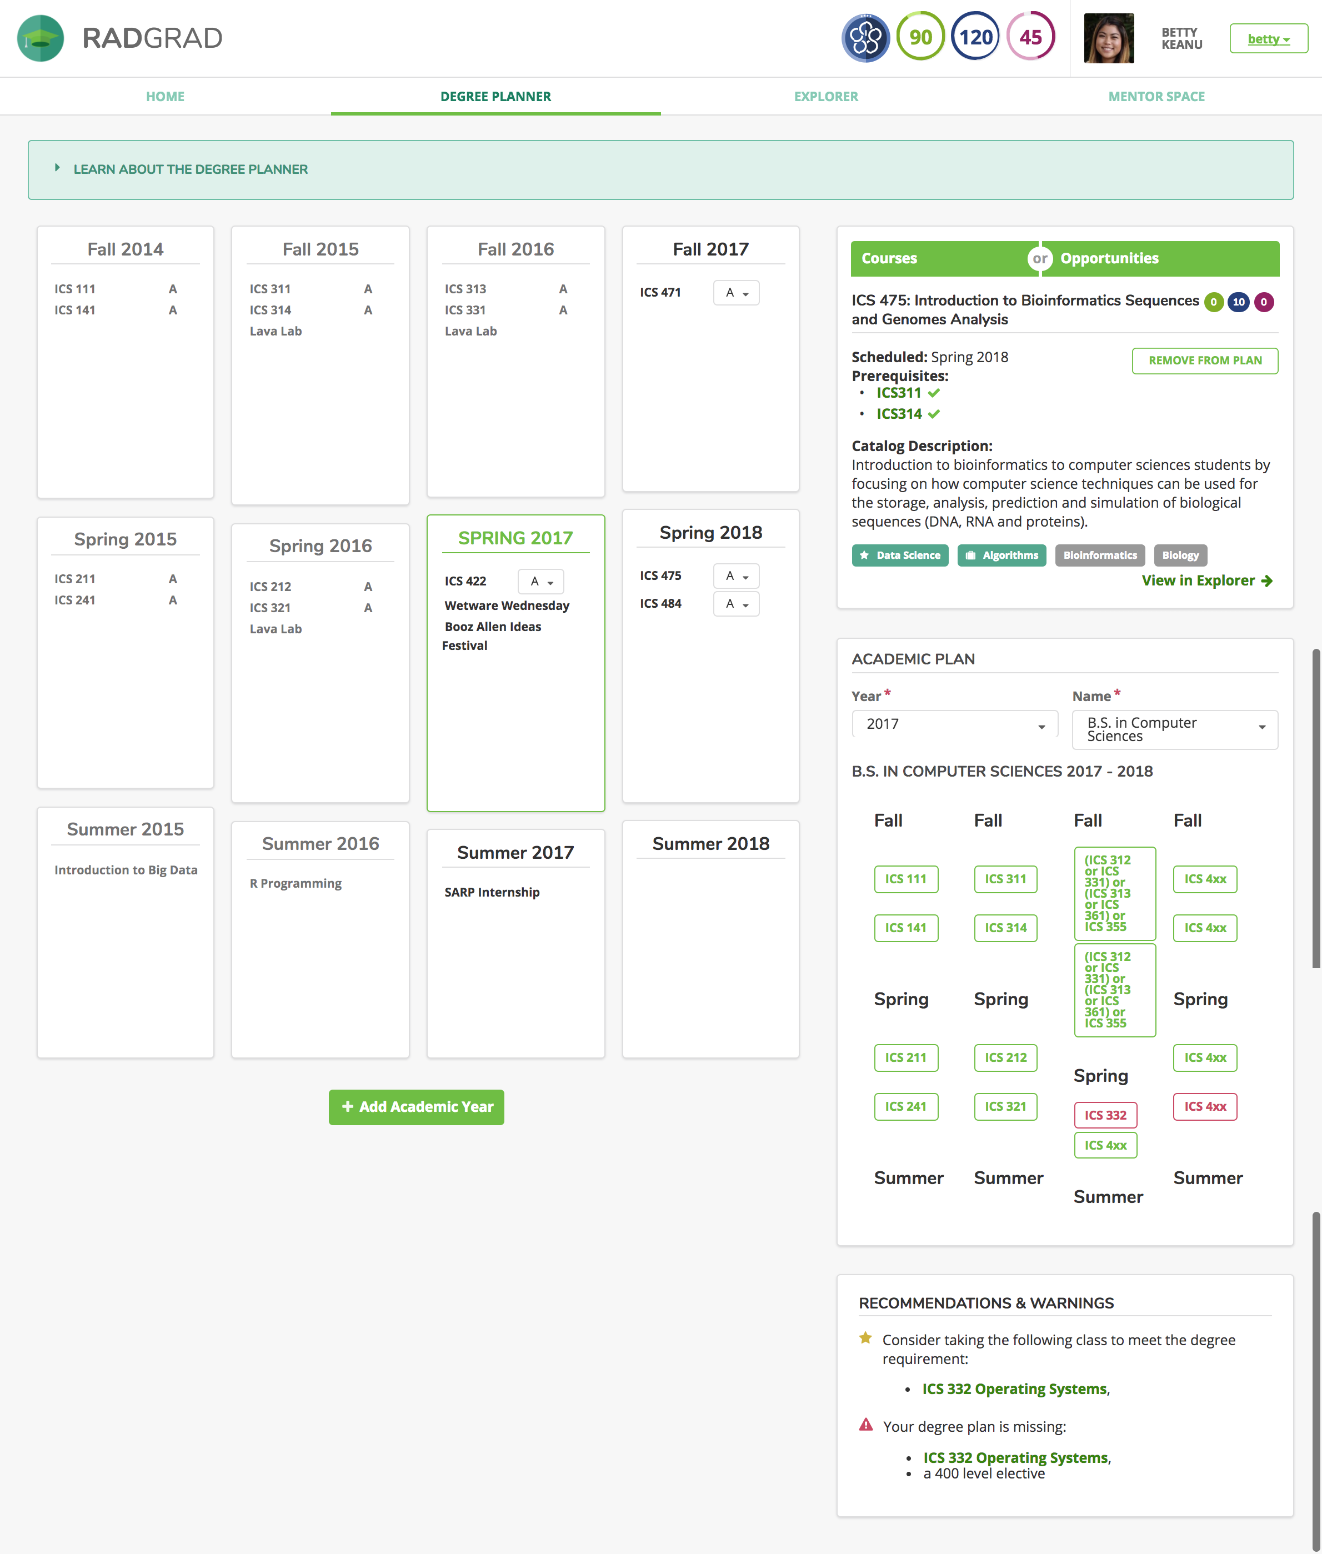
\includegraphics[width=1.0\textwidth]{degree-planner}
\caption{Degree planner page.}
\end{figure}

\begin{figure}[htbp!]
\centering
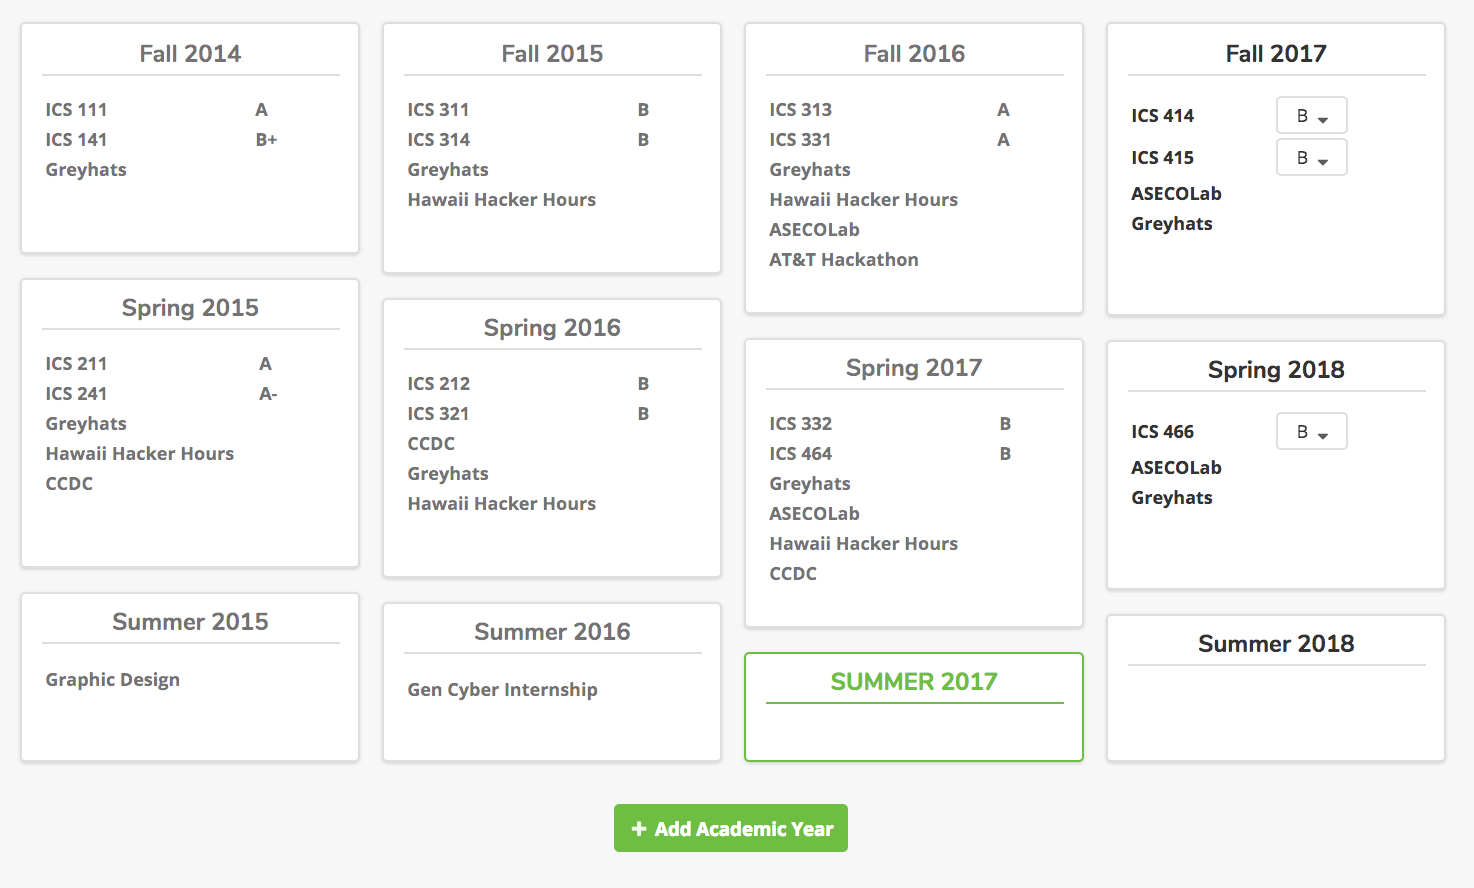
\includegraphics[width=1.0\textwidth]{dp-dp}
\caption{Close up of degree plan on the degree planner page.}
\end{figure}
The student degree planner was created to help students increase their extracurricular engagement in a way that makes sense for their specific path and fits into their time constraints (Figure 6.20, Figure 6.21). The student degree planner is the main place that students will go to view and make changes to their entire degree plan. Students can view up to four academic years at a time, but they can view additional past or future years by clicking on the green arrows at the bottom. Semesters that are in the past are greyed out and cannot be changed by the student. Any present or future semesters can be changed by dragging and dropping courses or opportunities into that semester pane. The grades for a course can be changed with the drop down menus. 

\begin{figure}[htbp!]
\centering
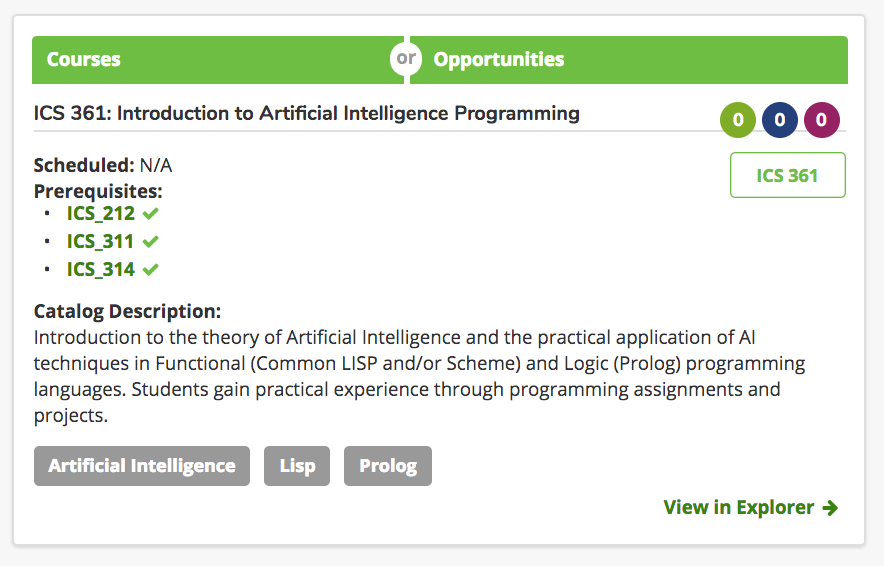
\includegraphics[width=1.0\textwidth]{dp-viewer}
\caption{Close up of the inspector on the degree planner page.}
\end{figure}

This page also includes an inspector pane on the top right hand corner, which the student can use to view brief details about a course or opportunity while planning their degree (Figure 6.20, Figure 6.22). The in-depth course and opportunity explorer pages can be accessed through the inspector, but the short descriptions in the inspector allows for quick and convenient assistance within the same view as the degree planner itself. The student can choose a course or opportunity to inspect by either choosing from the green dropdown menu at the top of the inspector, or by clicking on the course or opportunity name within the plan. 

\begin{figure}[htbp!]
\centering
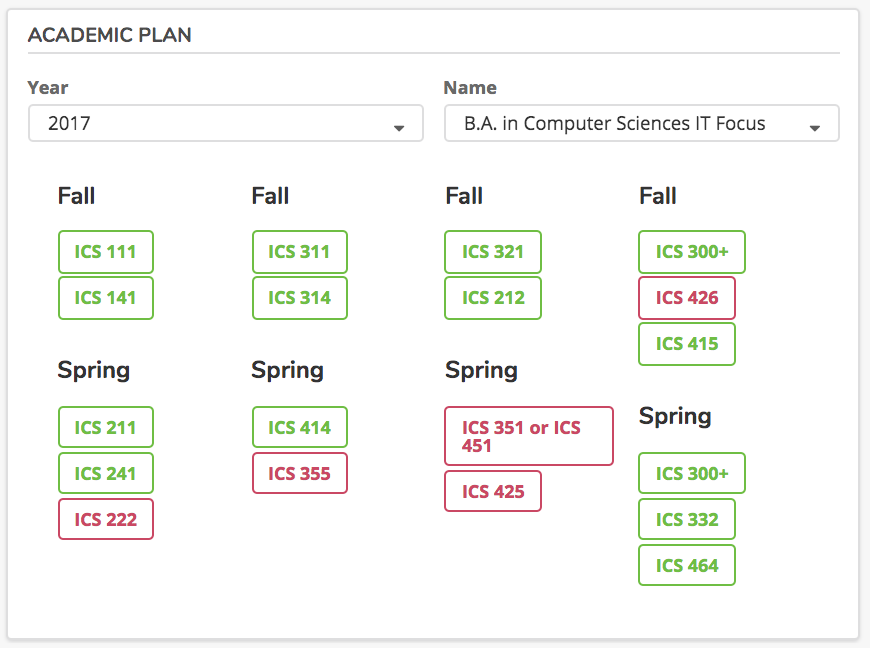
\includegraphics[width=1.0\textwidth]{dp-academicplan}
\caption{Close up of academic plans on the degree planner page.}
\end{figure}
Below the inspector is the academic plan pane (Figure 6.20, Figure 6.23). In this pane, students can select a year and an academic plan name (i.e. B.S. in Computer Science Security Science) to indicate the degree plan that the would like to follow. The pane then displays the required courses for this plan, organized into the recommended semesters, and color coded (green for classes in the student's plan, and red for classes not in the student's plan). Students can use this display to easily drag their missing courses onto their plan.


\subsubsection{Recommendations and Warnings}
\begin{figure}[htbp!]
\centering
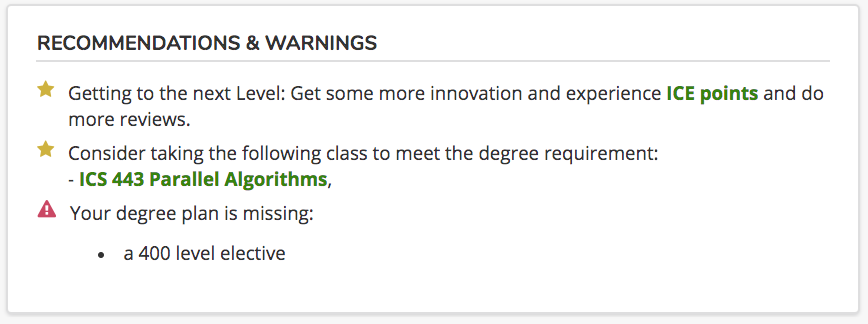
\includegraphics[width=1.0\textwidth]{dp-rw}
\caption{Close up of recommendations and warnings on the degree planner page.}
\end{figure}

The student degree planner automatically generates warnings and recommendations on the bottom right hand corner (Figure 6.20, Figure 6.24). These warnings and recommendations change as a student's degree plan changes. Each time a student adds, moves, or removes a course or opportunity through the degree planner, explorer, or student home page, the warnings and recommendations will regenerate. All possible warnings and recommendations as of June 2017 are listed in Table 6.4. These recommendations and warnings were created to help make the process of integrating courses and opportunities into a chosen time frame easier.

\begin{figure}[htbp!]
\centering
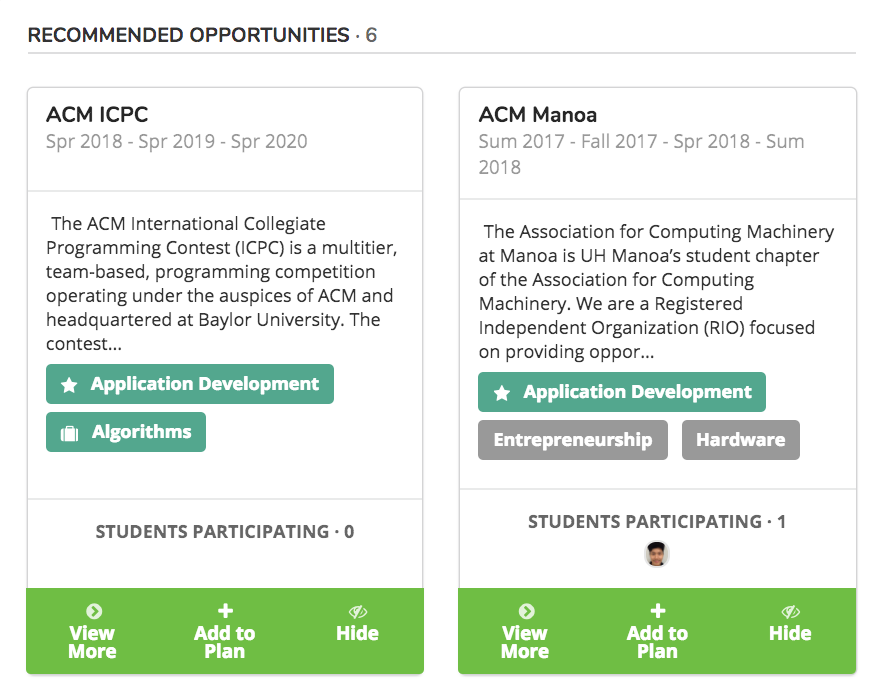
\includegraphics[width=1.0\textwidth]{home-recommend}
\caption{Close up of recommendations on the student home page.}
\end{figure}

On the student home page, students can see details about recommended courses and opportunities as soon as they log in (Figure 6.25, Figure 6.31). These are chosen based off the student's chosen interests and career goal related interests. If a student is interested in a particular course or opportunity, they can choose to view more in the explorer, add it to their plan, or leave it there to decide what to do with later. If a student knows they are not interested in a certain course or opportunity, they can choose to hide it by clicking the "hide" button. If the student later changes their mind, they can view and unhide the course or opportunity by clicking ``Hidden Opportunities." These home page recommendations were created to help make the process of choosing and integrating interesting courses and opportunities easier and less overwhelming.


\begin{table}[htbp!]
\centering
\begin{tabular}{  |p{8cm}|p{8cm}| } 
  \hline
 \textbf{Warnings} & \textbf{Recommendations} \\ 
  \hline
A prerequisite course is missing & Course recommended based upon interests\\
\hline
Semester appears overloaded (more than 3 ICS courses) & Opportunity recommended based upon interests\\
\hline
A required course is missing & Recommendation for ICS innovation points \\
\hline
Course is not offered in chosen semester (future implementation) & Recommendation for ICS competency points \\
\hline
& Recommendation for ICS experience points\\
\hline
& Move towards achieving the next level \\
\hline
& See your ICS advisor to upload STAR data\\
 \hline
\end{tabular}
\caption{Automatically generated warnings and recommendations as of May 2017}
\label{table:4}
\end{table}

\subsubsection{Career Goal, Course, Desired Degree and Opportunity Explorers}
Students can access the career goal, course, desired degree, and opportunity explorers to help them plan their degree.  These explorers can be accessed through the ``Explorer" top menu on the student home page. The specific explorer can be chosen using the dropdown menu on the left side. These explorers were created to help make the process of combining career goals, courses, degrees, and opportunities together into a cohesive degree plan faster and easier. Students can go to one place to find all of the information they need to piece their plan together, rather than having to depend on a number of external sources..

\begin{figure}[htbp!]
\centering
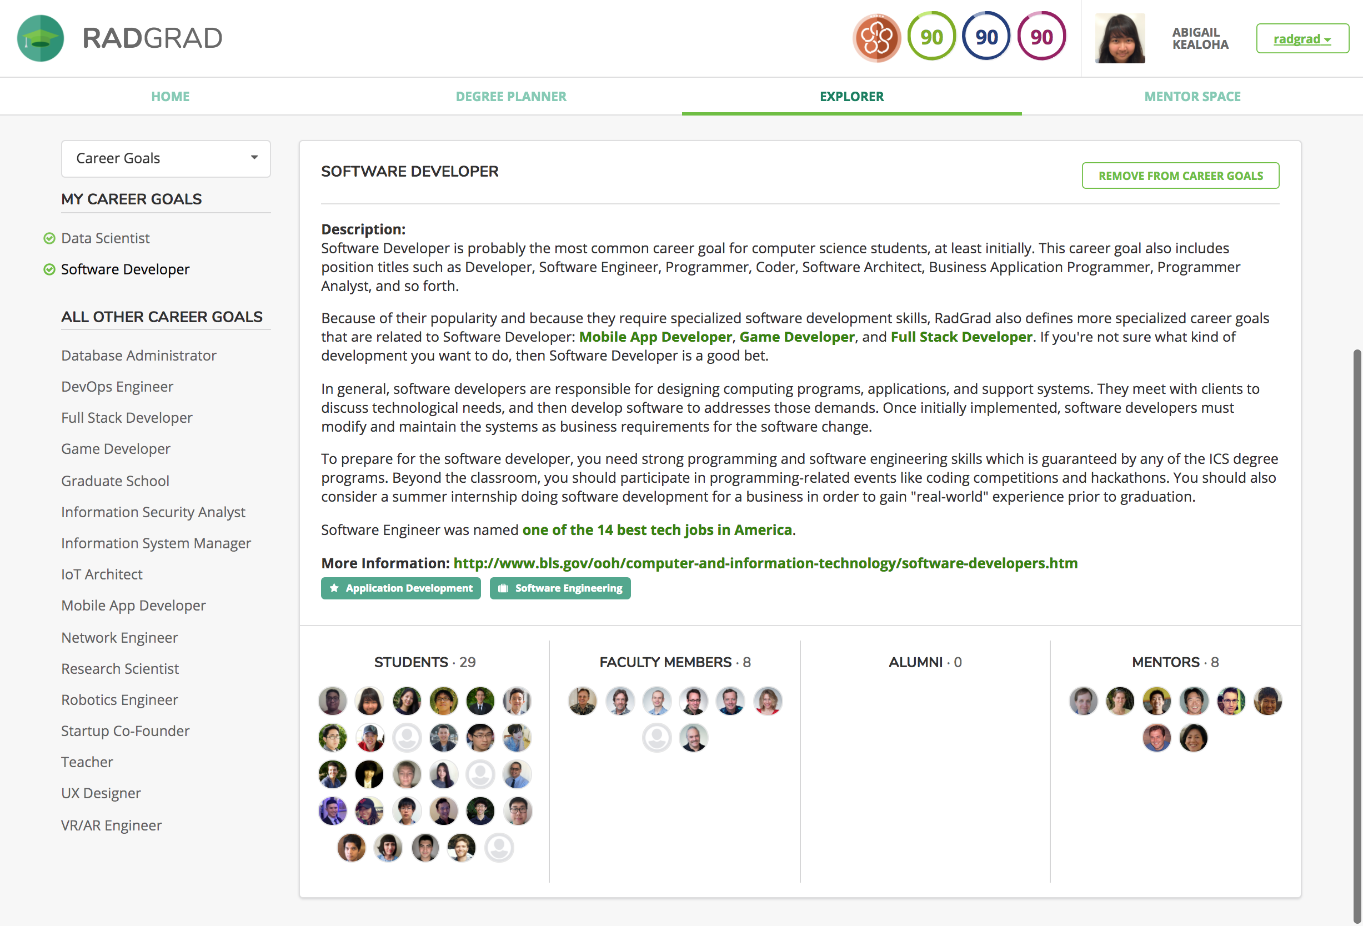
\includegraphics[width=1.0\textwidth]{careergoal-explorer}
\caption{Career goal explorer page.}
\end{figure}

The career goal explorer lists all RadGrad career goals on the left side (Figure 6.26). These career goals are arranged by ``My Career Goals" (career goals that the user has added) and ``All other career goals" (career goals that the user has not added). The user can click on a career goal to view details about that career goal. These details include a description of the career goal, related interests, related courses and/or opportunities, a link for more information, interested students, interested faculty, interested alumni, and interested mentors. On this page, the user can also add or remove the career goal by clicking on the green button at the top right corner.  

\begin{figure}[htbp!]
\centering
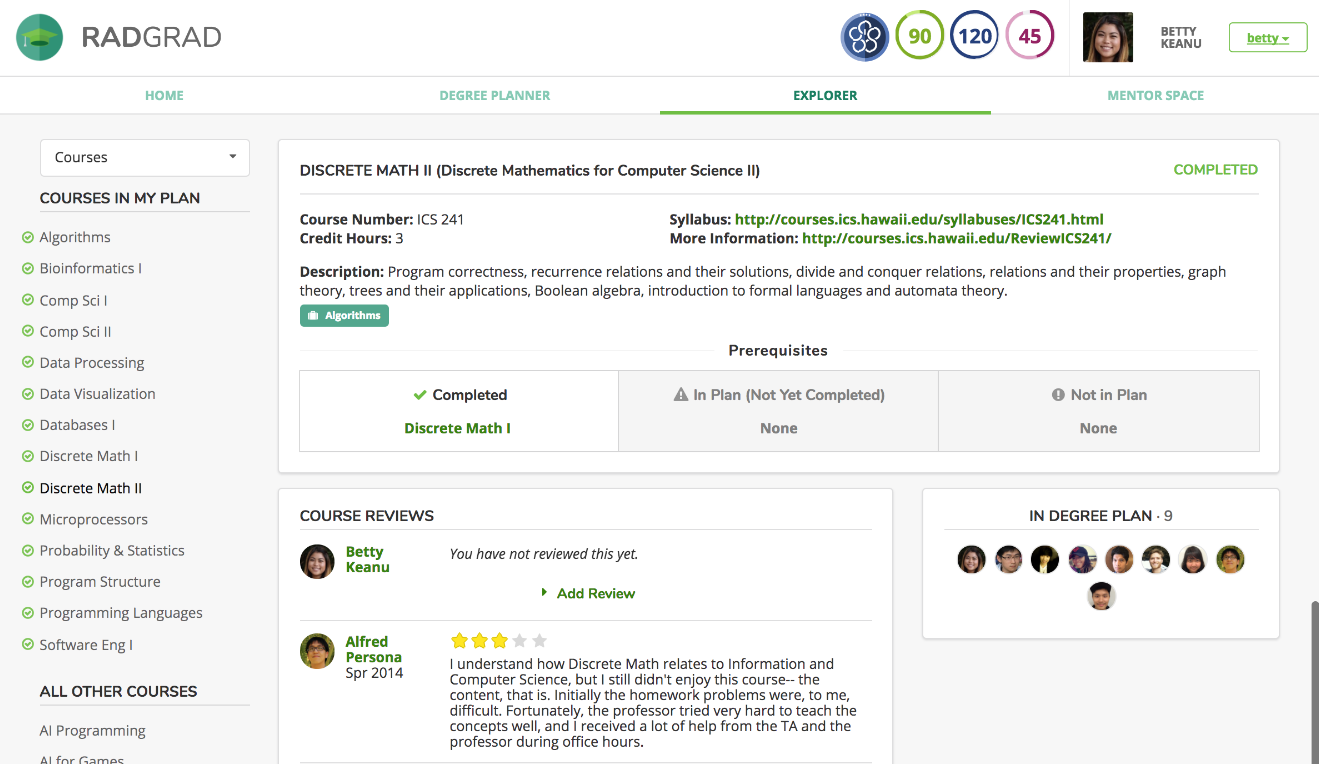
\includegraphics[width=1.0\textwidth]{course-explorer}
\caption{Course explorer page.}
\end{figure}

The course explorer lists all RadGrad courses on the left side (Figure 6.27). These courses are arranged by ``Courses in my Plan" (all past, present or future courses in the student's degree plan) and ``All Other Courses" (courses not in the user's degree plan). The user can click on a course to view details about that course. These details include course number, a link to the syllabus, credit hours, a description of the course, prerequisites, organized into three categories (completed, in plan but not yet completed, and not in plan), and a list of students with this course in their degree plan. On this page, users can also view course reviews from other students and add or edit their own course review. The user can add or remove this course from their degree plan by clicking on the green button at the top right corner. If the user has already taken and passed the course, they cannot add it again.

\begin{figure}[htbp!]
\centering
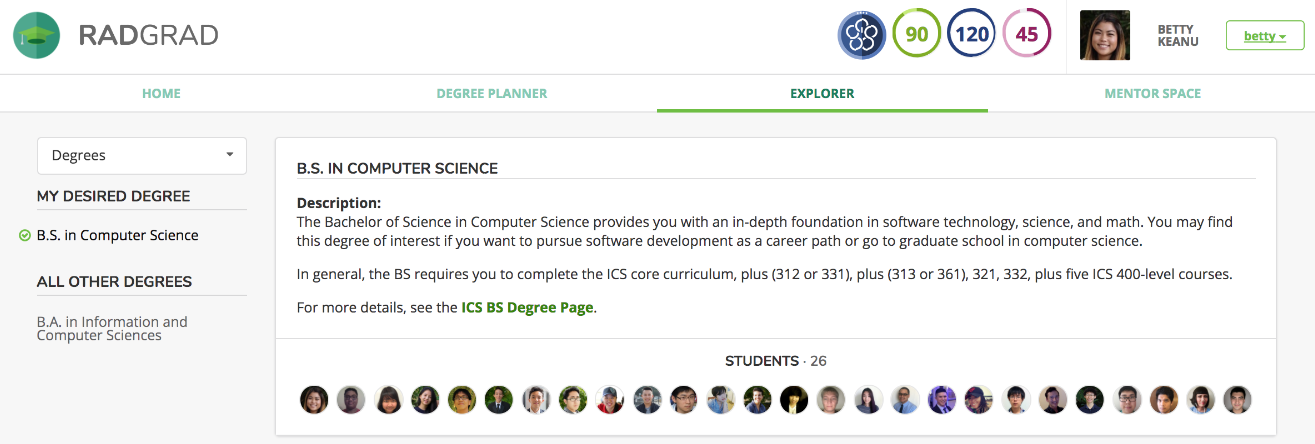
\includegraphics[width=1.0\textwidth]{degree-explorer}
\caption{Degree explorer page.}
\end{figure}

The degree explorer lists all possible ICS degrees on the left side (Figure 6.28). These degrees are arranged by ``My Desired Degree" (the student can only have one desired degree at a time), and ``All Other Degrees" (degrees not currently chosen as the user's desired degree). The user can click on a degree to view details about that degree. These details include a description, where to go for more information, and a list of students who have this degree listed as their current desired degree. On this page, users can set a new degree goal by clicking on the green button at the top right corner.

\begin{figure}[htbp!]
\centering
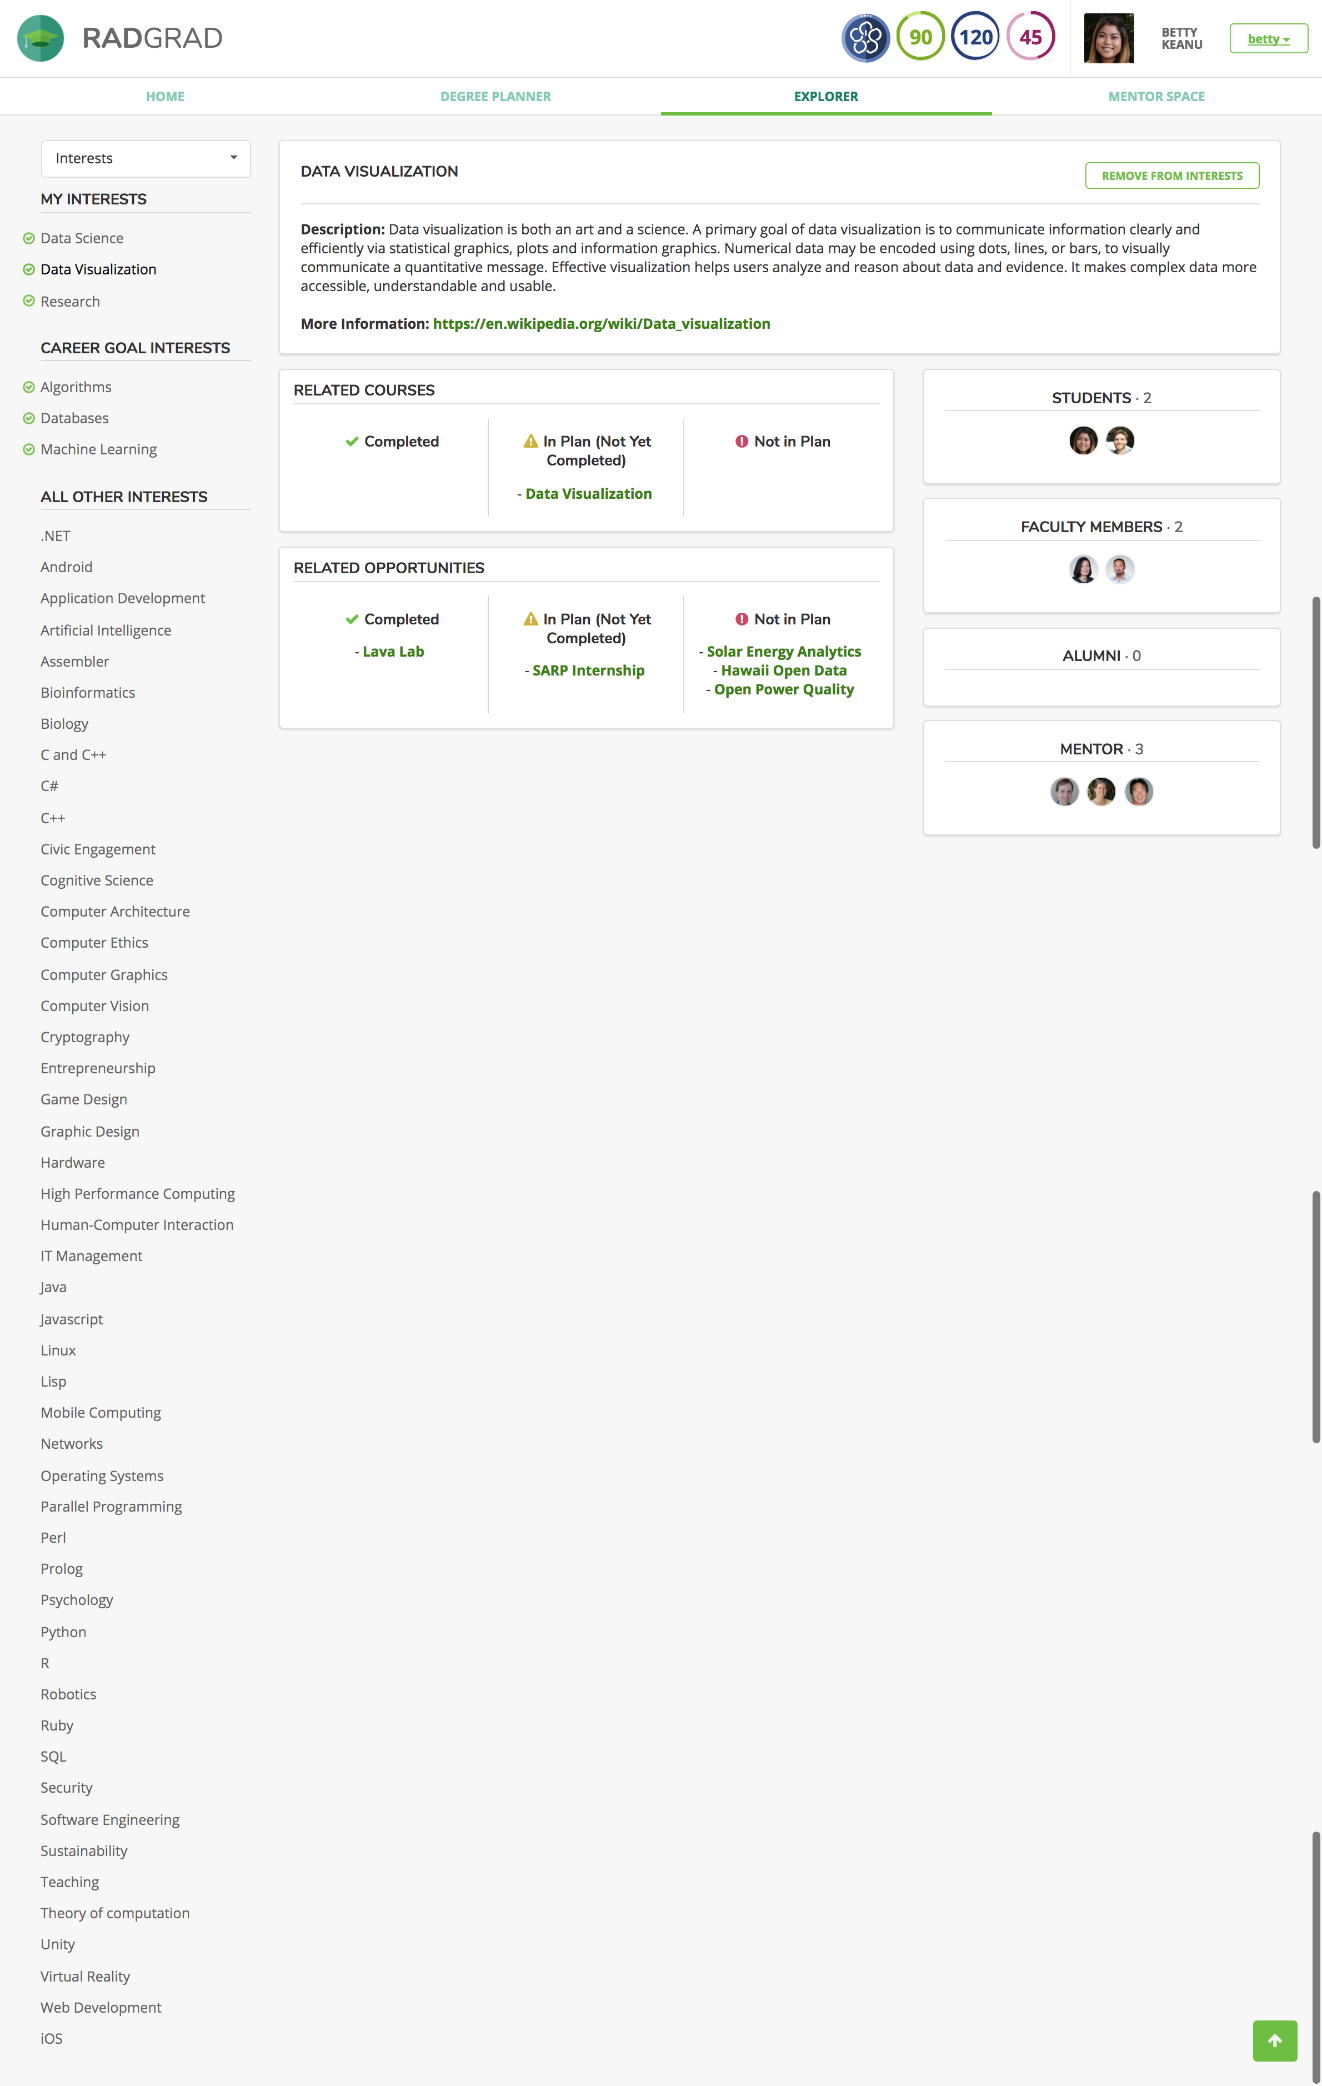
\includegraphics[width=1.0\textwidth]{interest-explorer}
\caption{Interest explorer page.}
\end{figure}

The interest explorer lists all possible RadGrad interests on the left side (Figure 6.29). These interests are arranged by ``My Interests" (interests that the user has added), ``Career Goal Interests" (interests that have automatically been added due to their association with one or more of the user's chosen career goals), and ``All Other Interests" (interests that the user has not added and are not related to any of the user's career goals). The user can click on an interest to view details about that interest. These details include a description of the interest, related courses and related opportunities, both organized into three categories (completed, in plan but not yet completed, and not in plan), and students, faculty, alumni, and mentors who have added this interest. On this page, users can also add or remove the interest by clicking on the green button at the top right corner.

\begin{figure}[htbp!]
\centering
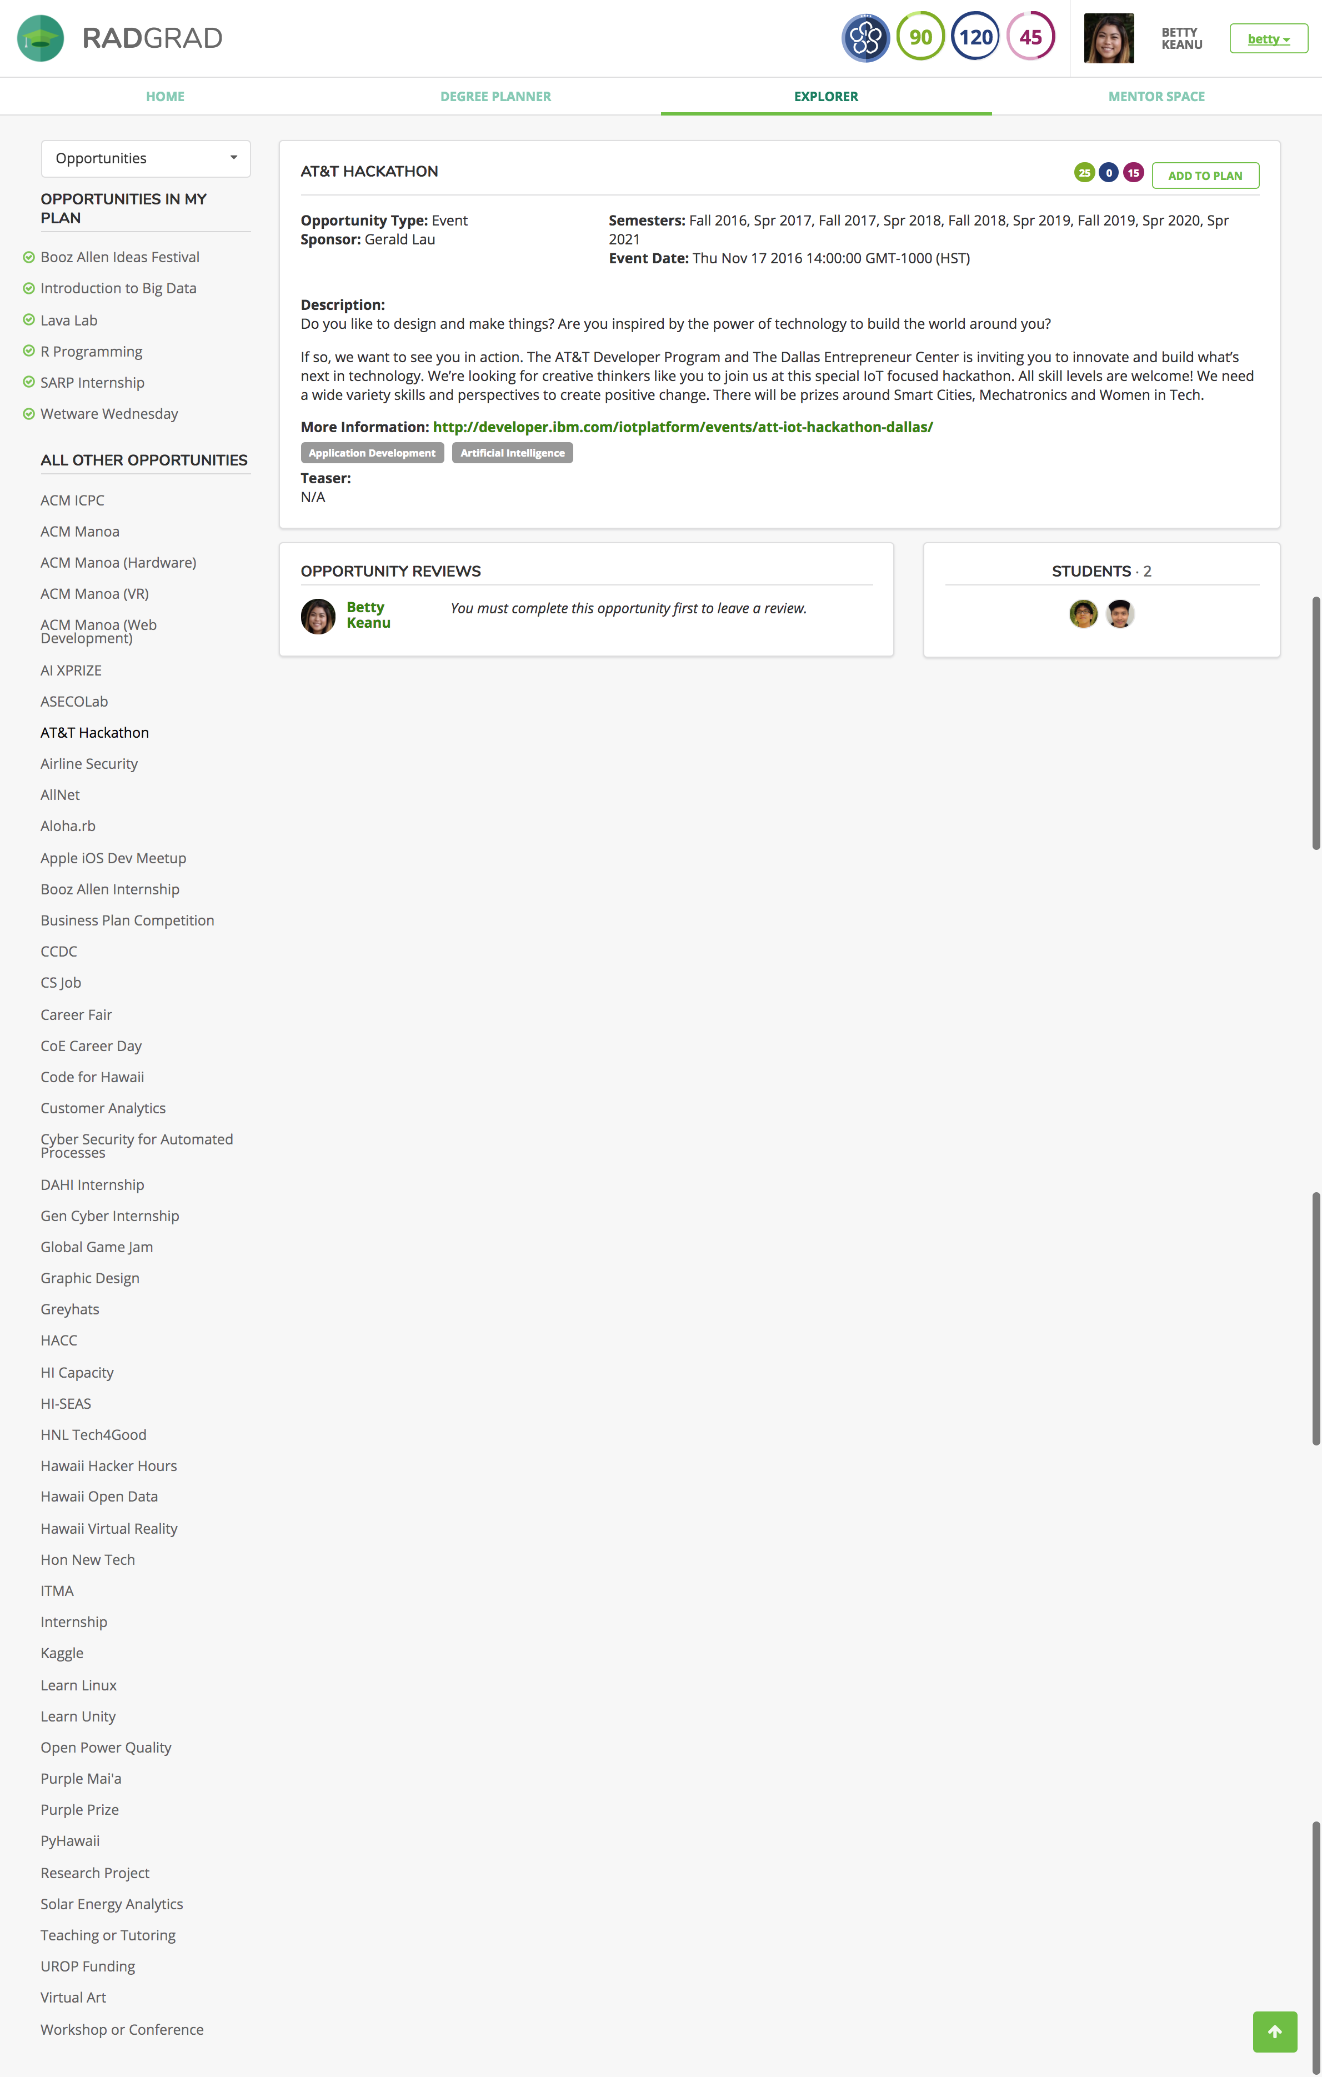
\includegraphics[width=1.0\textwidth]{opportunity-explorer}
\caption{Opportunity explorer page.}
\end{figure}

The opportunity explorer lists all ICS opportunities on the left side (Figure 6.30). These opportunities are arranged by ``Opportunities in my Plan" (all past, present or future opportunities in the user's degree plan) and ``All Other Opportunities" (opportunities not in the user's degree plan). The user can click on an opportunity to view details about that opportunity. These details include the opportunity type, semesters offered, event date, faculty sponsor, a description of the opportunity, related interests, a teaser video, and a list of students with this opportunity in their degree plan. On this page, users can also view opportunity reviews from other students and add or edit their own opportunity review. The user can add or remove this opportunity from their degree plan by clicking on the green button at the top right corner. Unlike courses, users can add an opportunity to their plan as many times as they would like.

\begin{figure}[htbp!]
\centering
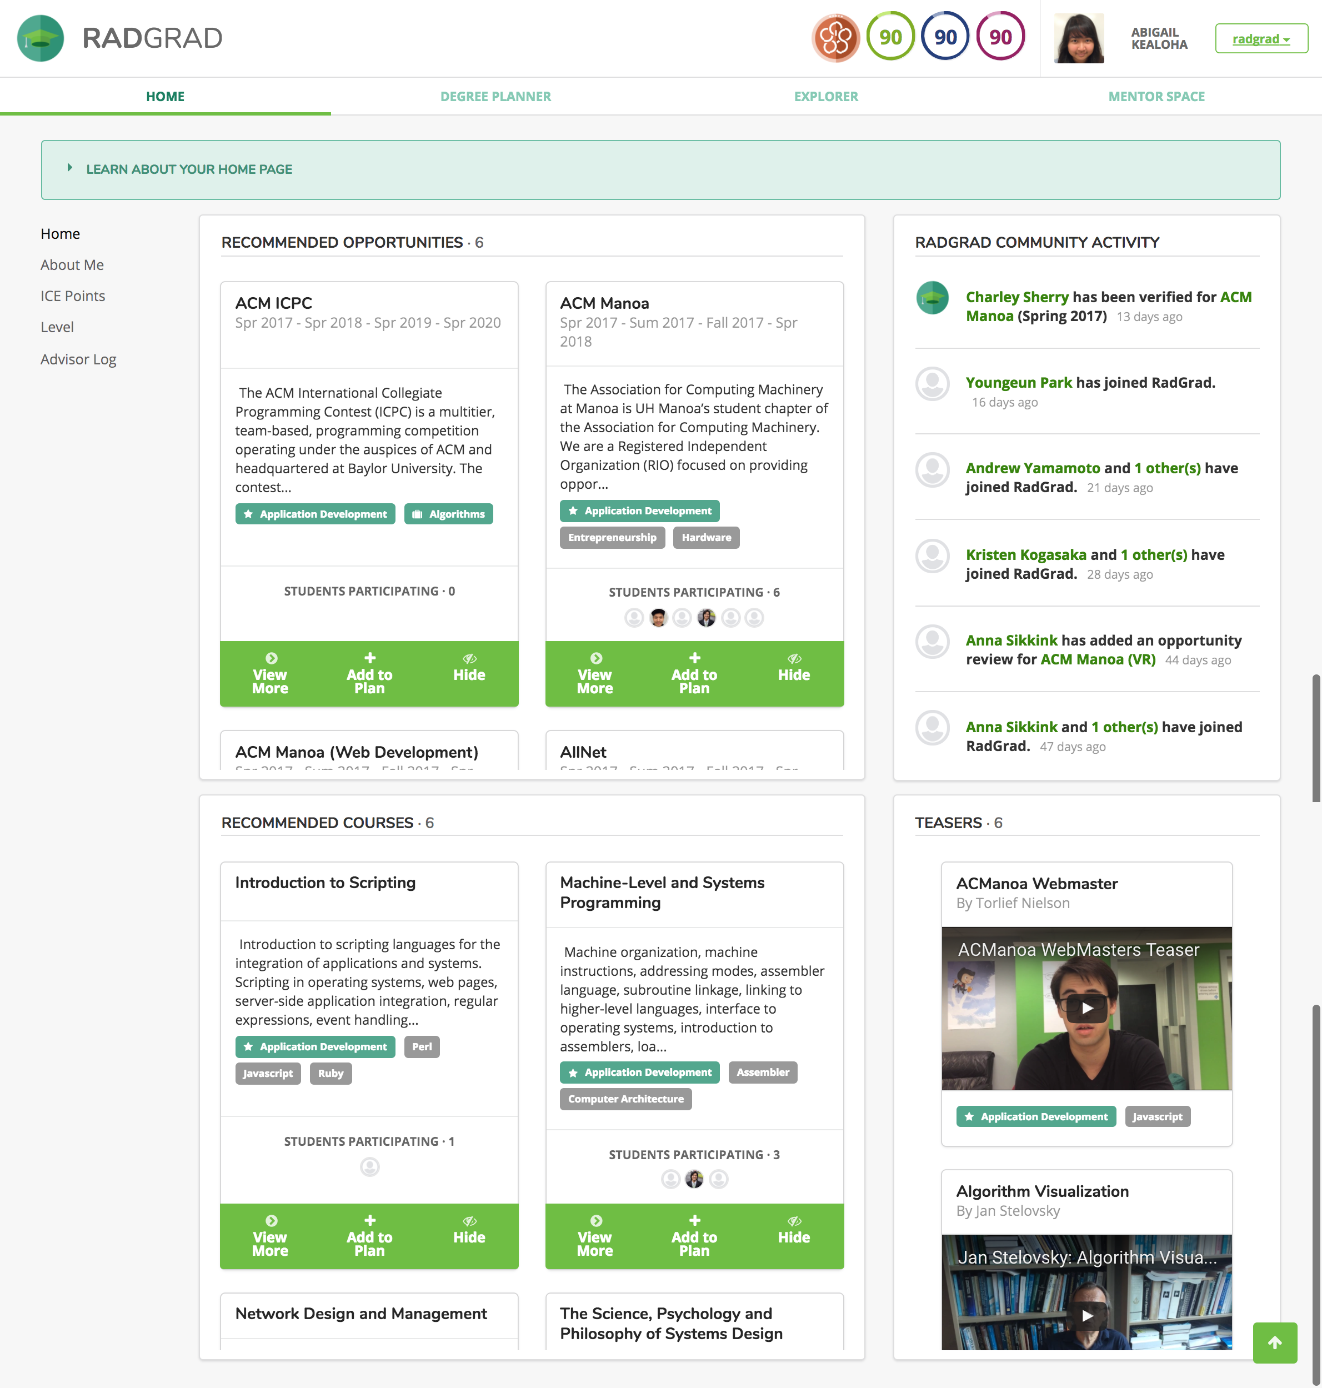
\includegraphics[width=1.0\textwidth]{student-home}
\caption{Student home page with teasers, feed, and recommended courses and opportunities.}
\end{figure}

\subsubsection{Teasers}
\begin{figure}[htbp!]
\centering
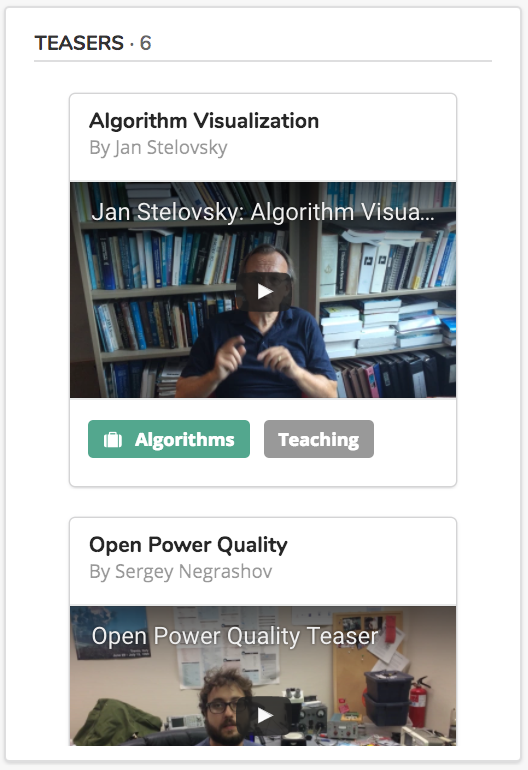
\includegraphics[width=0.5\textwidth]{teaser-widget}
\caption{Close up of teasers on student home page.}
\end{figure}
Teasers are short (around 30 seconds) YouTube videos created by members of RadGrad to advertise their opportunity to the rest of RadGrad (Figure 6.32, Figure 6.31). Faculty members can create a teaser to help give students an idea of what their current research is about, and students can create a teaser to help give students an idea of what their club or event does and why other students should participate. These teasers supplement the textual opportunity descriptions in the explorer, and appear on the student's home page based off matching interests. Teasers were added on the student home page to serve as eye catching advertisements for opportunities, specifically targeted towards the user.

\subsection{Social Network}
\subsubsection{Avatars}
\begin{figure}[htbp!]
\centering
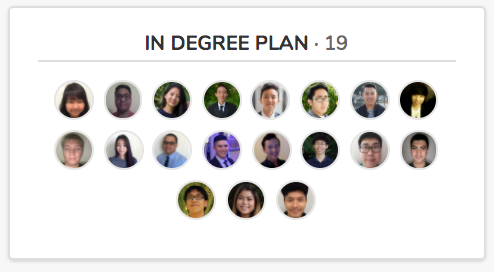
\includegraphics[width=0.5\textwidth]{avatar}
\caption{Example of avatars on the course explorer page.}
\end{figure}
RadGrad quietly reminds users that they are not alone in using the system--they are part of a large and diverse network of real people (Figure 6.33). One of the ways RadGrad does this is by incorporating user avatars around the site. These avatars appear on the student home page, explorer pages, the user explorer, the student levels page, and the MentorSpace page. These avatars appear to show users related to a certain interest, career goal, course, opportunity, degree, and level. They also are associated with feed items, reviews, and MentorSpace answers. All avatars can be clicked on to navigate to the user's profile in the user explorer.  

\subsubsection{Feed}
\begin{figure}[htbp!]
\centering
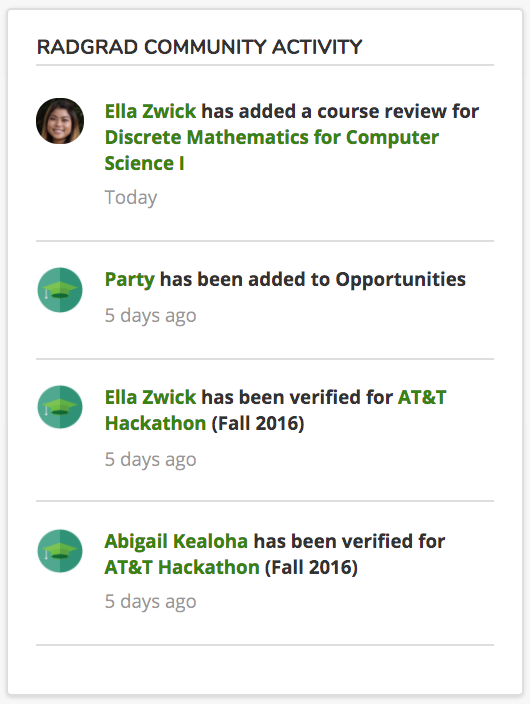
\includegraphics[width=0.5\textwidth]{feed}
\caption{Close up of feed on student home page.}
\end{figure}
Another way RadGrad reminds users that they are not alone in using the system is by providing a feed on the student home page (Figure 6.34, Figure 6.31). The feed is one of the first things that a user sees when they log in. Through this feed, users can see events occurring throughout RadGrad such as a new user joining RadGrad, a new course or opportunity is added on RadGrad, a user is verified for an opportunity, or a user has written a new course or opportunity review. The feed provides a single place for students to go to when they want to see what has changed since they have last logged in, and it constantly keeps students updated with the latest changes to the system. Since the feed also allows students to see what other students have been doing, they may be able to get a quick sense of what opportunities are popular among their classmates.

\subsubsection{Mentorspace}
\begin{figure}[htbp!]
\centering
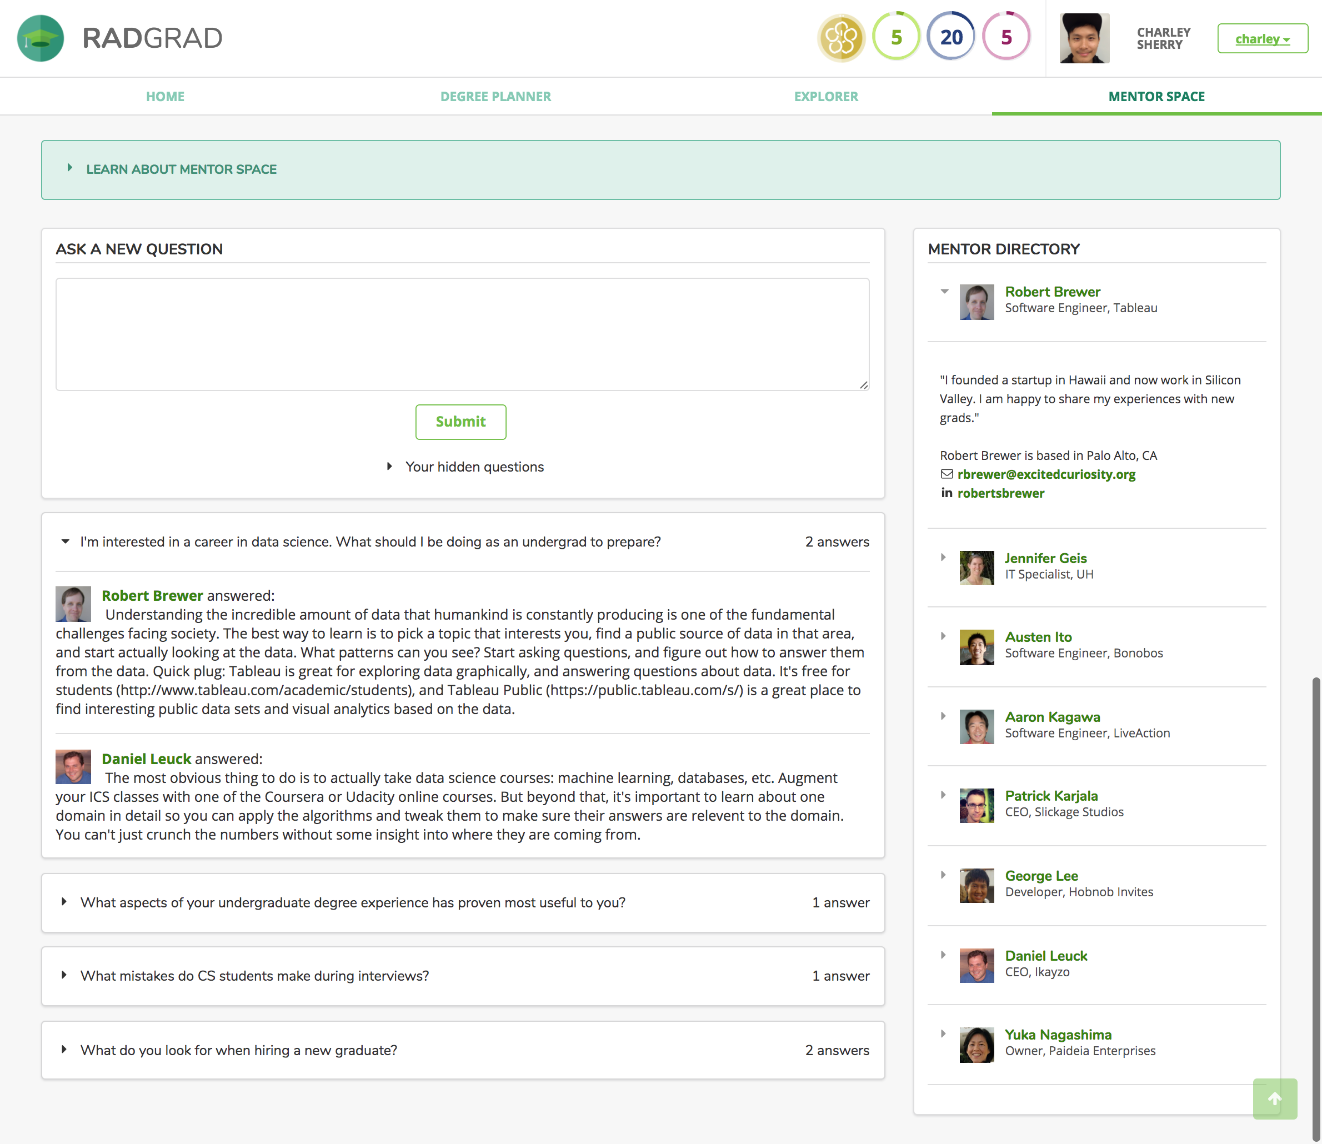
\includegraphics[width=1.0\textwidth]{mentor-space}
\caption{MentorSpace page.}
\end{figure}
Mentors and students can interact with each other on the MentorSpace page (Figure 6.35). MentorSpace was created to encourage more academic and professional interactions between students and alumni. The mentors are listed in the Mentor Directory on the right side of the page. Students can explore who the mentors are by expanding their profile and viewing information about their current company, current location, current job title, email address, LinkedIn, and a description about what inspired them to become a RadGrad mentor. On the left side of the page, students can submit new questions that they have for a mentor. Once the question has gone through moderation (by  Administrators), it will be posted on the MentorSpace for everyone to see. If a question is rejected, it can be edited and resubmitted as many times as desired. A question may be rejected if it contains profanity, is unclear, or is unrelated to ICS. Once a question is posted, mentors can leave an answer for the rest of the community to see. If a student has a specific question for a specific mentor, they can instead contact the mentor through the provided email rather than posting on MentorSpace, which is reserved for questions that can benefit the general ICS student community. 

\subsubsection{Advisor Log}
\begin{figure}[htbp!]
\centering
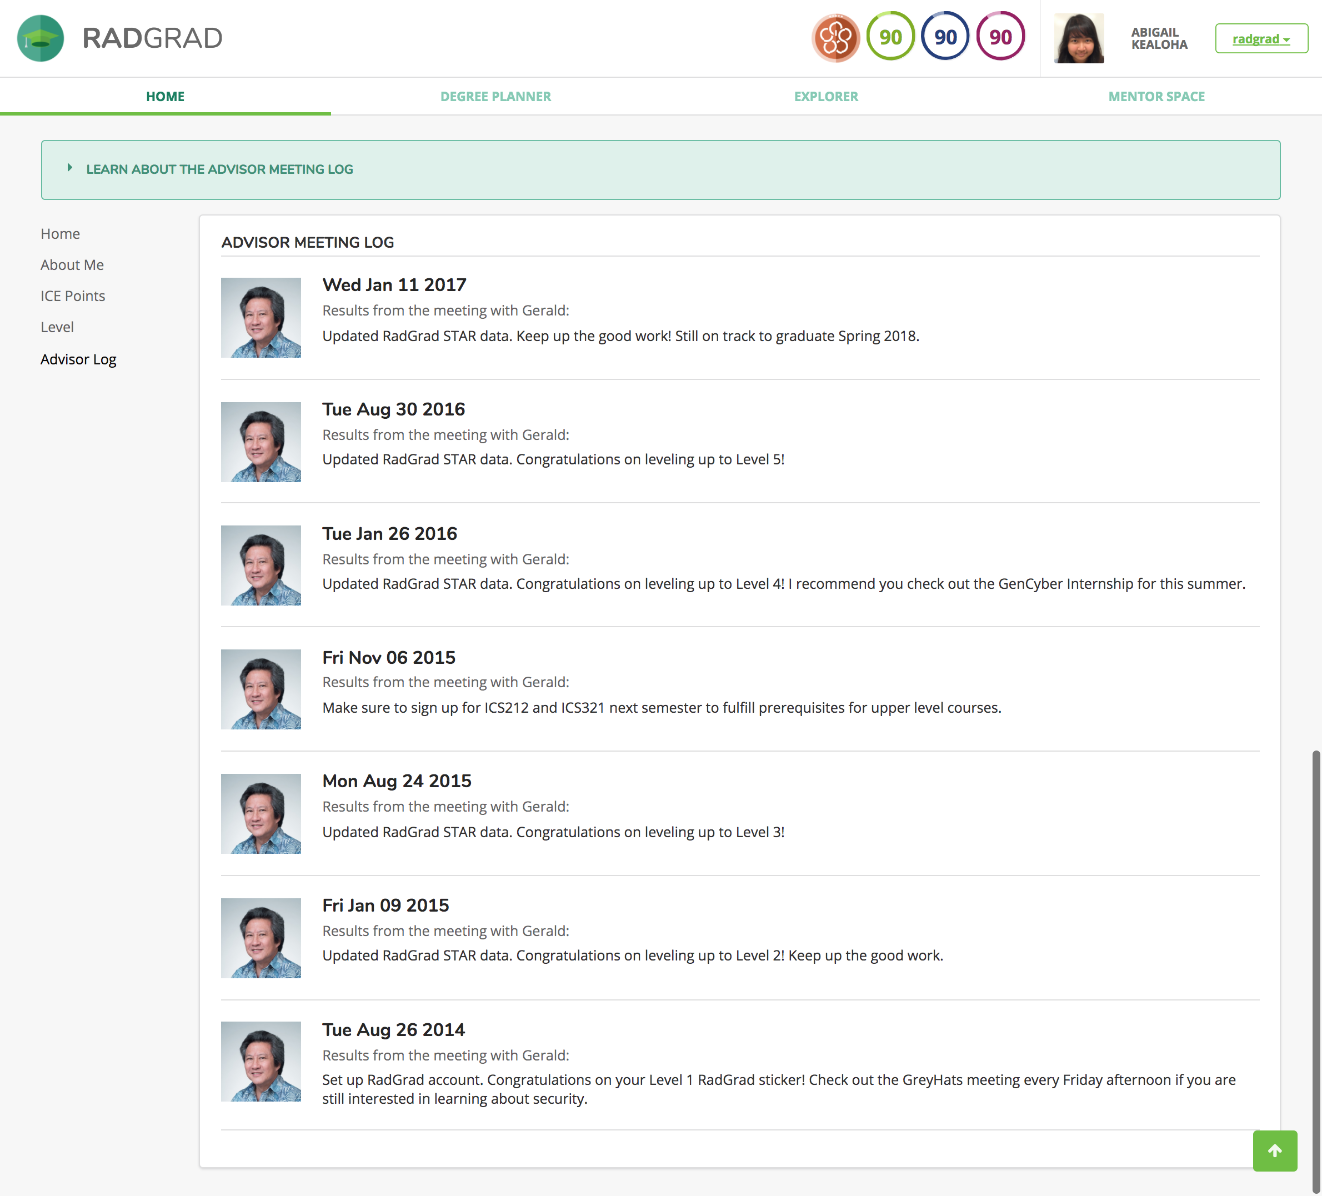
\includegraphics[width=1.0\textwidth]{advisor-log}
\caption{Student advisor log page.}
\end{figure}
Advisors and students can interact with each other on the Advisor Log page (Figure 6.36). Advisor logs were created to help encourage and augment the interactions between students and advisors. When an advisor holds a meeting with a student, he can leave notes from the meeting on the student's Advisor Log. Each log includes a date, the name and avatar of the advisor, and the meeting notes. Advisors can use the log to keep track of their interactions with each student, and students can refer back to the log whenever they can't remember details about what their advisor had said. 

\subsubsection{Reviews}
\begin{figure}[htbp!]
\centering
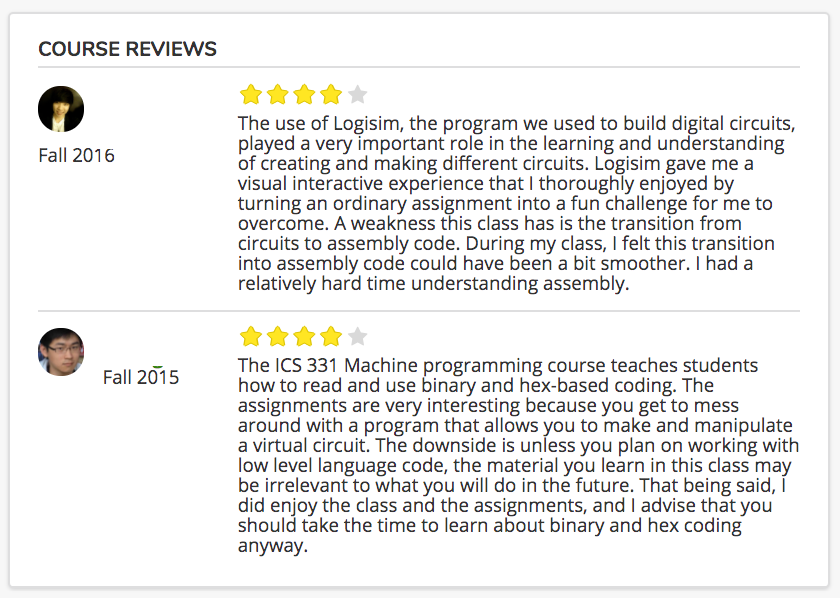
\includegraphics[width=0.5\textwidth]{reviews}
\caption{Close up of reviews on the course explorer page.}
\end{figure}
Students can post two different types of reviews: course reviews and opportunity reviews (Figure 6.37). Students can leave reviews for a specific course or opportunity on the course or opportunity explorer page. Students can leave a 1-5 rating and reasons behind their rating. Students can edit or delete their review at any time. Any new or edited reviews immediately appear on the explorer page, but when they go through moderation, they may be removed if they do not abide by the guidelines. Reviews cannot be anonymous, which forces students to take full responsibility for whatever they decide to post. This, along with the fact that all users on RadGrad can view reviews, allows for full transparency between professors and students. Students can view other students reviews to get additional, first hand and anecdotal information about a course or opportunity before they decide to add it to their plan. Faculty and advisors can view reviews to gather feedback about how to improve the ICS program. Reviews encourage more open communication between students and the rest of the RadGrad community.

\subsubsection{User Explorer}
\begin{figure}[htbp!]
\centering
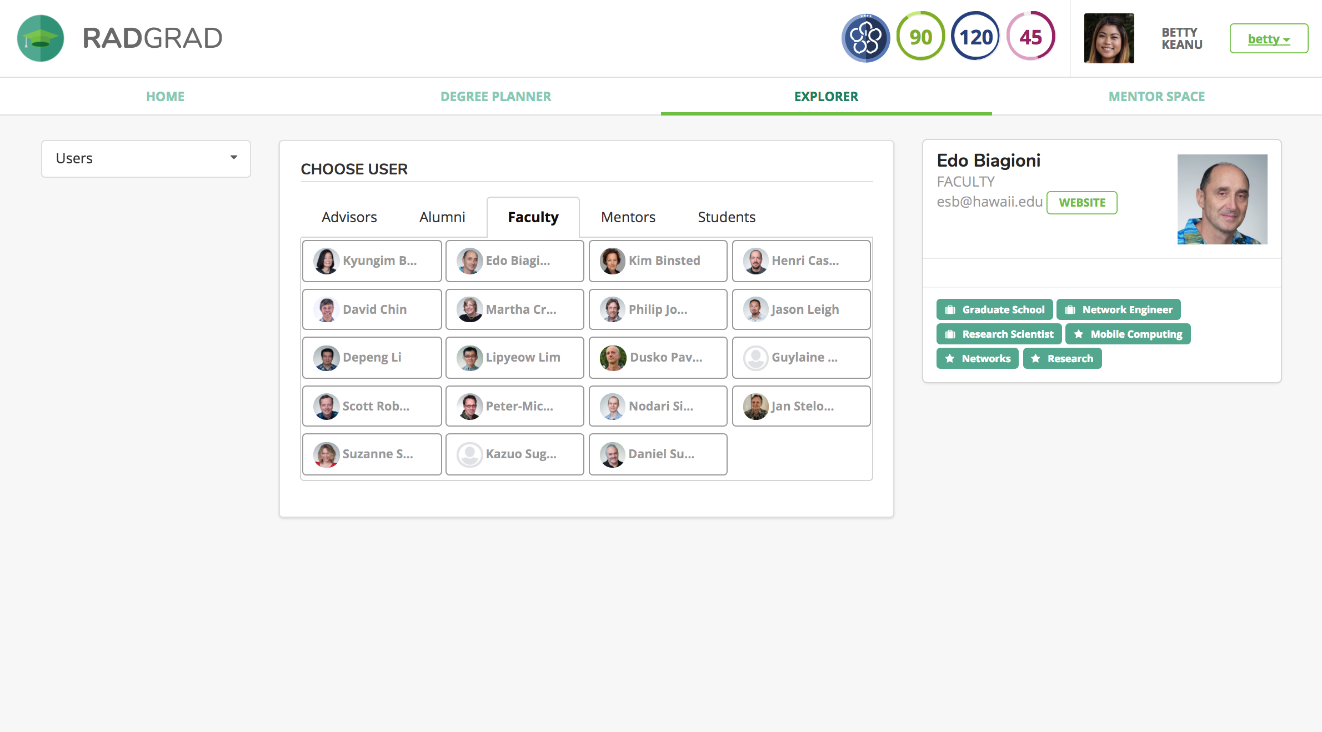
\includegraphics[width=1.0\textwidth]{user-explorer-faculty}
\caption{User explorer page.}
\end{figure}

The user explorer lists all RadGrad users with their first name, last name, and avatar (Figure 6.38). Users are arranged in tabs by user type (Advisor, Alumni, Faculty, Mentor, Student) and then listed alphabetically by last name. The current user can click on a user to view details about that user. For student users, these details include desired degree, email, level, taken and planned courses, and completed and planned opportunities. For faculty users, these details include their email, a link to their website, and interests. For mentor users, these details include their email, their MentorSpace answers, and their interests. For advisor users, these details include their email and their interests. Students can use this explorer to learn more about other members of the RadGrad community, and figure out who might be beneficial to talk to (i.e. a higher level student with matching interests and interesting completed opportunities, or a faculty member with matching interests, or a mentor working at the student's dream company). The User explorer was created to encourage more and better social interactions among all members of the RadGrad community.

\subsection{Gamification}
\subsubsection{ICE}
\begin{figure}[htbp!]
\centering
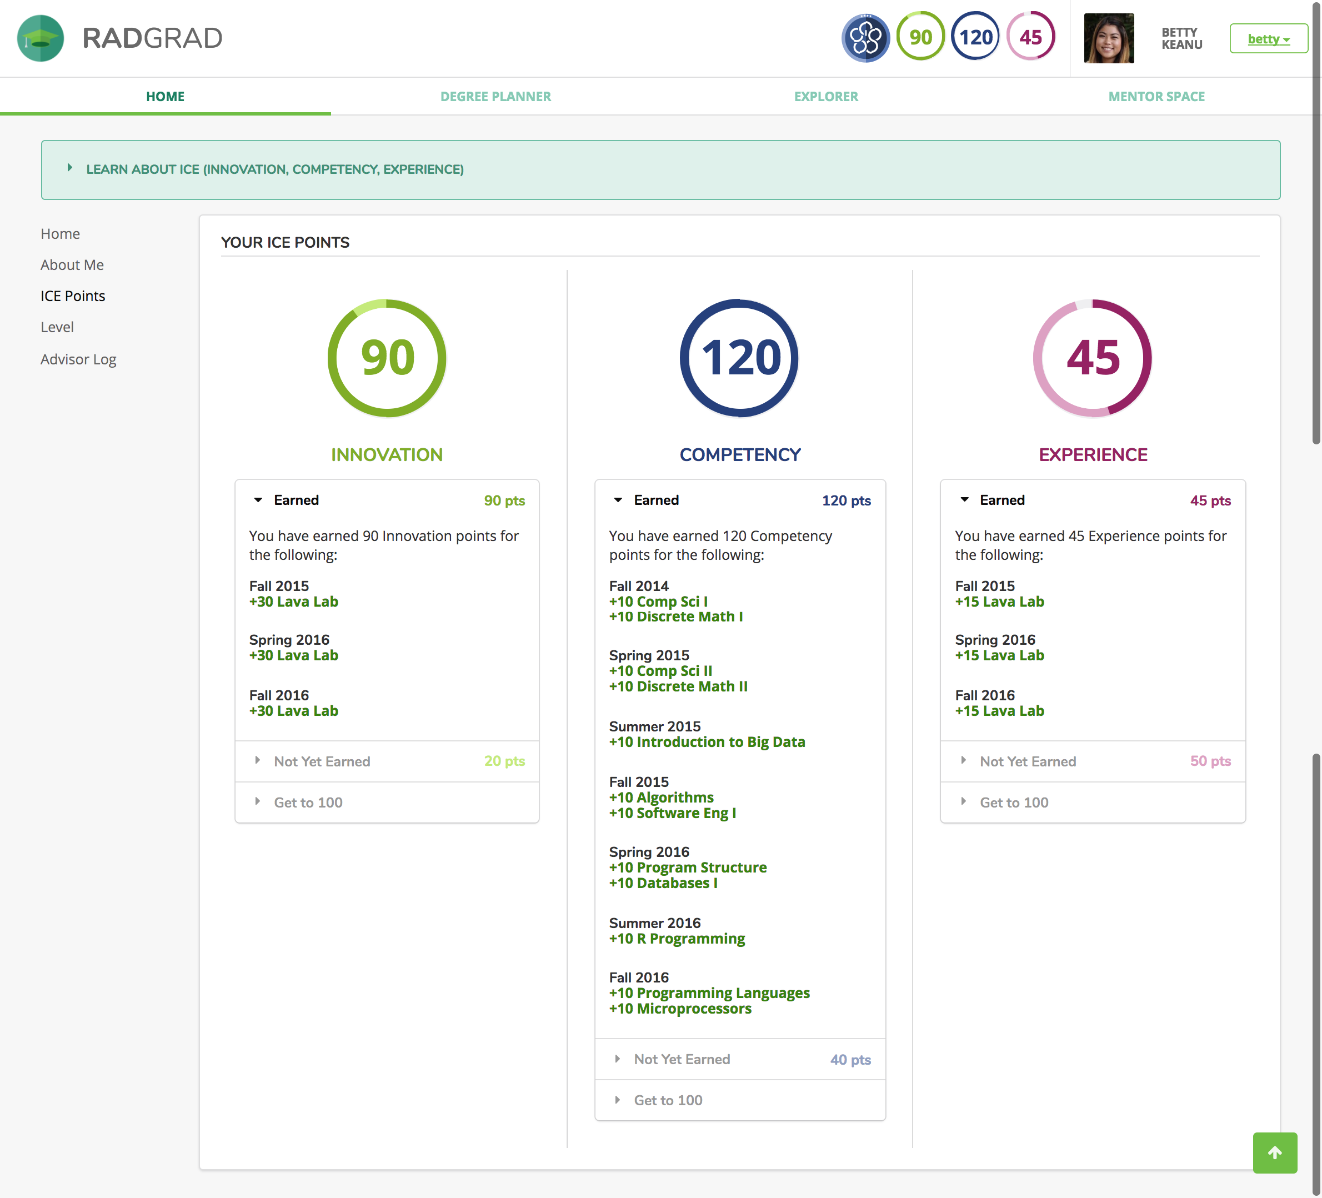
\includegraphics[width=1.0\textwidth]{student-ice}
\caption{ICE page.}
\end{figure}

The student ICE page displays three circular graphs: one each for innovation, competency, and experience (Figure 6.39). The number in the center of each graph represents the current amount of points earned for that category. The dark fill in the graph represents the same number. The light fill on the graph represents the amount of planned points. In addition to the student ICE page, these ICE graphs also appear in the top right corner of the menu bar. 

ICE points are also represented for specific courses or opportunities. These ICE points are represented using three filled circles: one each for innovation, competency, and experience. Each circle has a number in the center which represents the amount of points that course or opportunity is worth for that particular ICE category. Students can use these ICE representations to decide which courses or opportunities they should add to their plan, in order to improve their ICE score. These representations appear on the degree planner inspector pane and in the course and opportunity explorer pages. ICE is incorporated in multiple places all over the site to emphasize the importance of well-roundedness, with equal emphasis on innovation, competency, and experience.

\subsubsection{Levels}
\begin{figure}[htbp!]
\centering
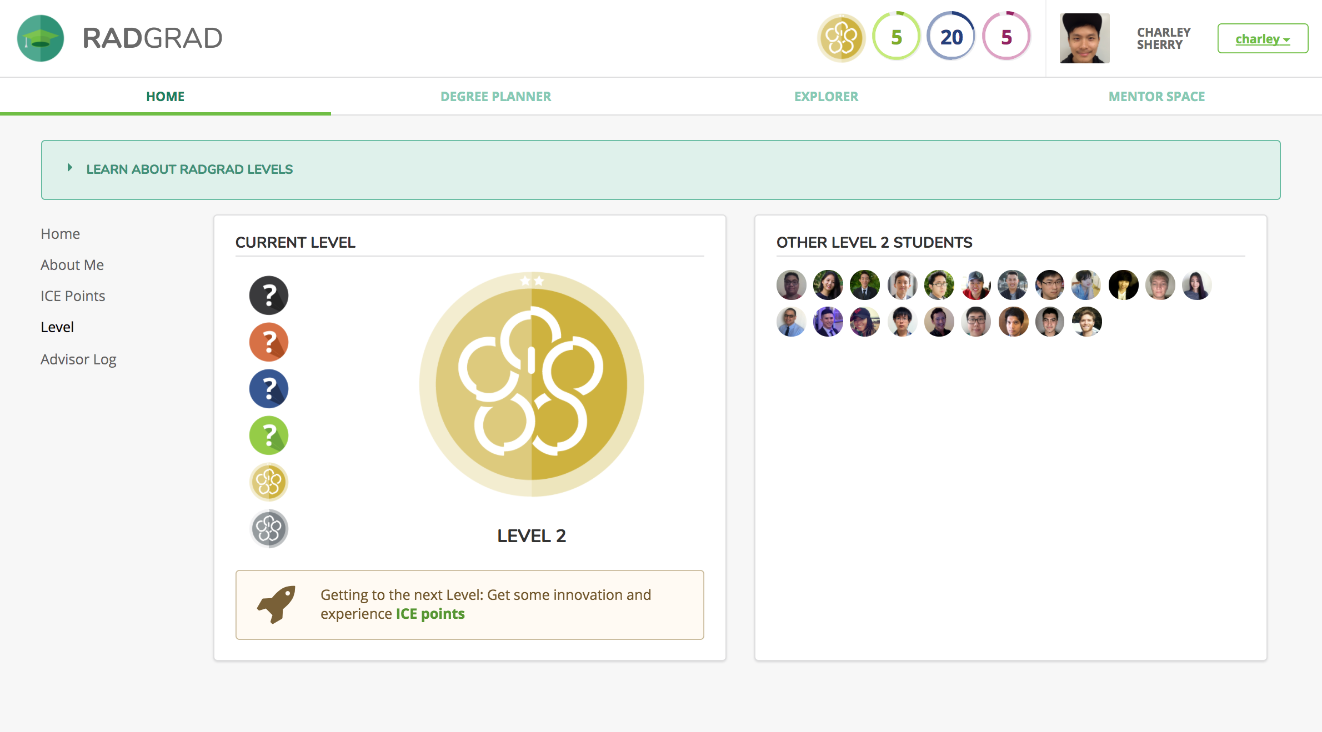
\includegraphics[width=1.0\textwidth]{levels}
\caption{Levels page.}
\end{figure}

Students can view their current level badge on the student level page (Figure 6.40). This page also includes leveling up hints and a list of other students who are at the same level (listed with avatars). This levels page was created to help students to feel a sense of progression throughout their program, and to help them to get to know their peers at the same level.

Levels also persist physically off of RadGrad in the form of stickers. These stickers can be obtained from an advisor or a RadGrad administrator, and a student will receive a new sticker each time they achieve a new level. Students are encouraged to display these stickers on their laptop, as a subtle way to communicate their current standing to their classmates. Using these stickers, students can more easily identify students who are at the same level as them to mingle with, identify students at a higher level than them to get advice from, and identify students at a lower level who could use some peer mentoring. These stickers can also be used to identify current or former ICS students while off campus. In this way, these physical manifestations of RadGrad help to create a sense of ICS community offline as well. 

\section{Advisor Mode}
\subsection{Student Configuration}
\begin{figure}[htbp!]
\centering
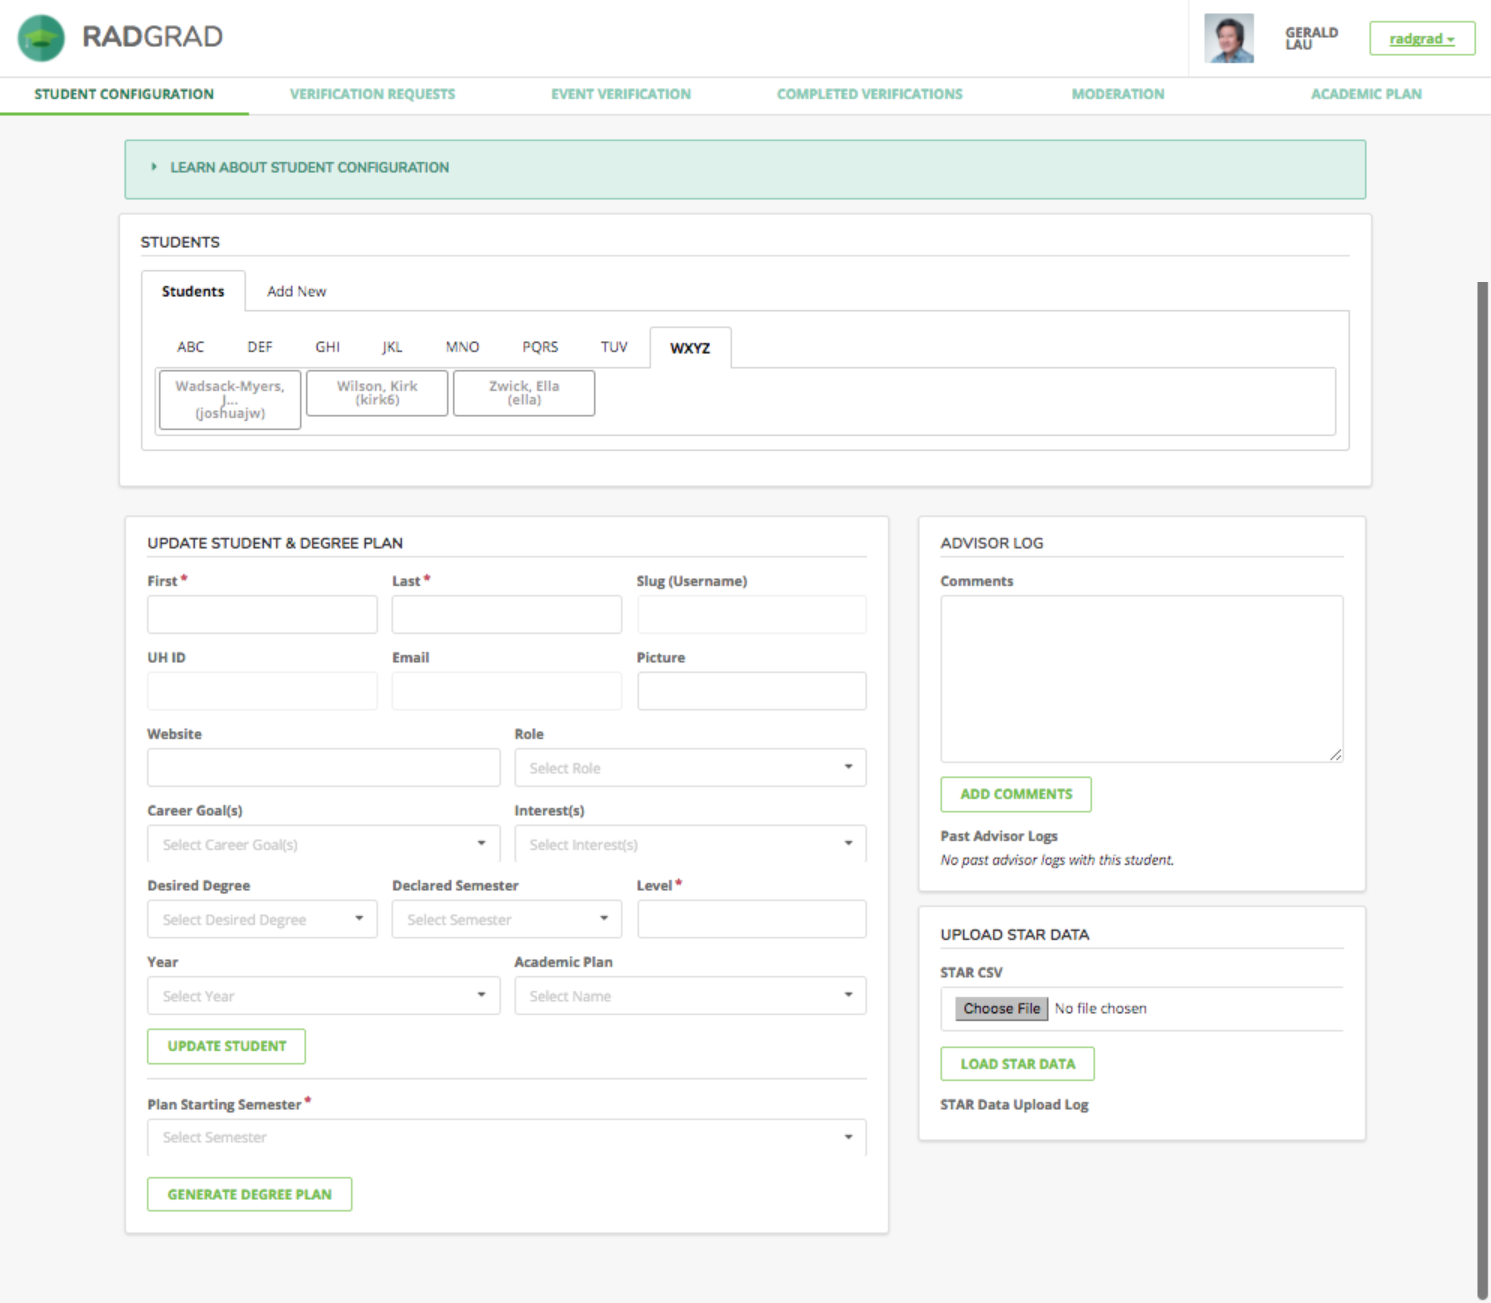
\includegraphics[width=1.0\textwidth]{advisor-student-configuration}
\caption{Advisor student configuration page.}
\end{figure}
On the student configuration page, advisors can add new students or update existing students (Figure 6.41). Existing students are listed alphabetically by last name. Advisors can update a student's first name, last name, picture, website, role, career goals, interests, desired degree, declared semester, level, year, academic plan, and plan starting semester from this interface. (Slug, email, and UH ID cannot be changed once the student has been added to RadGrad). On this page, advisors can also add advisor log comments and view any past advisor logs for a particular student. Advisors can also use this page to upload new star data and view past star data uploads. 
\subsection{Verification}
\begin{figure}[htbp!]
\centering
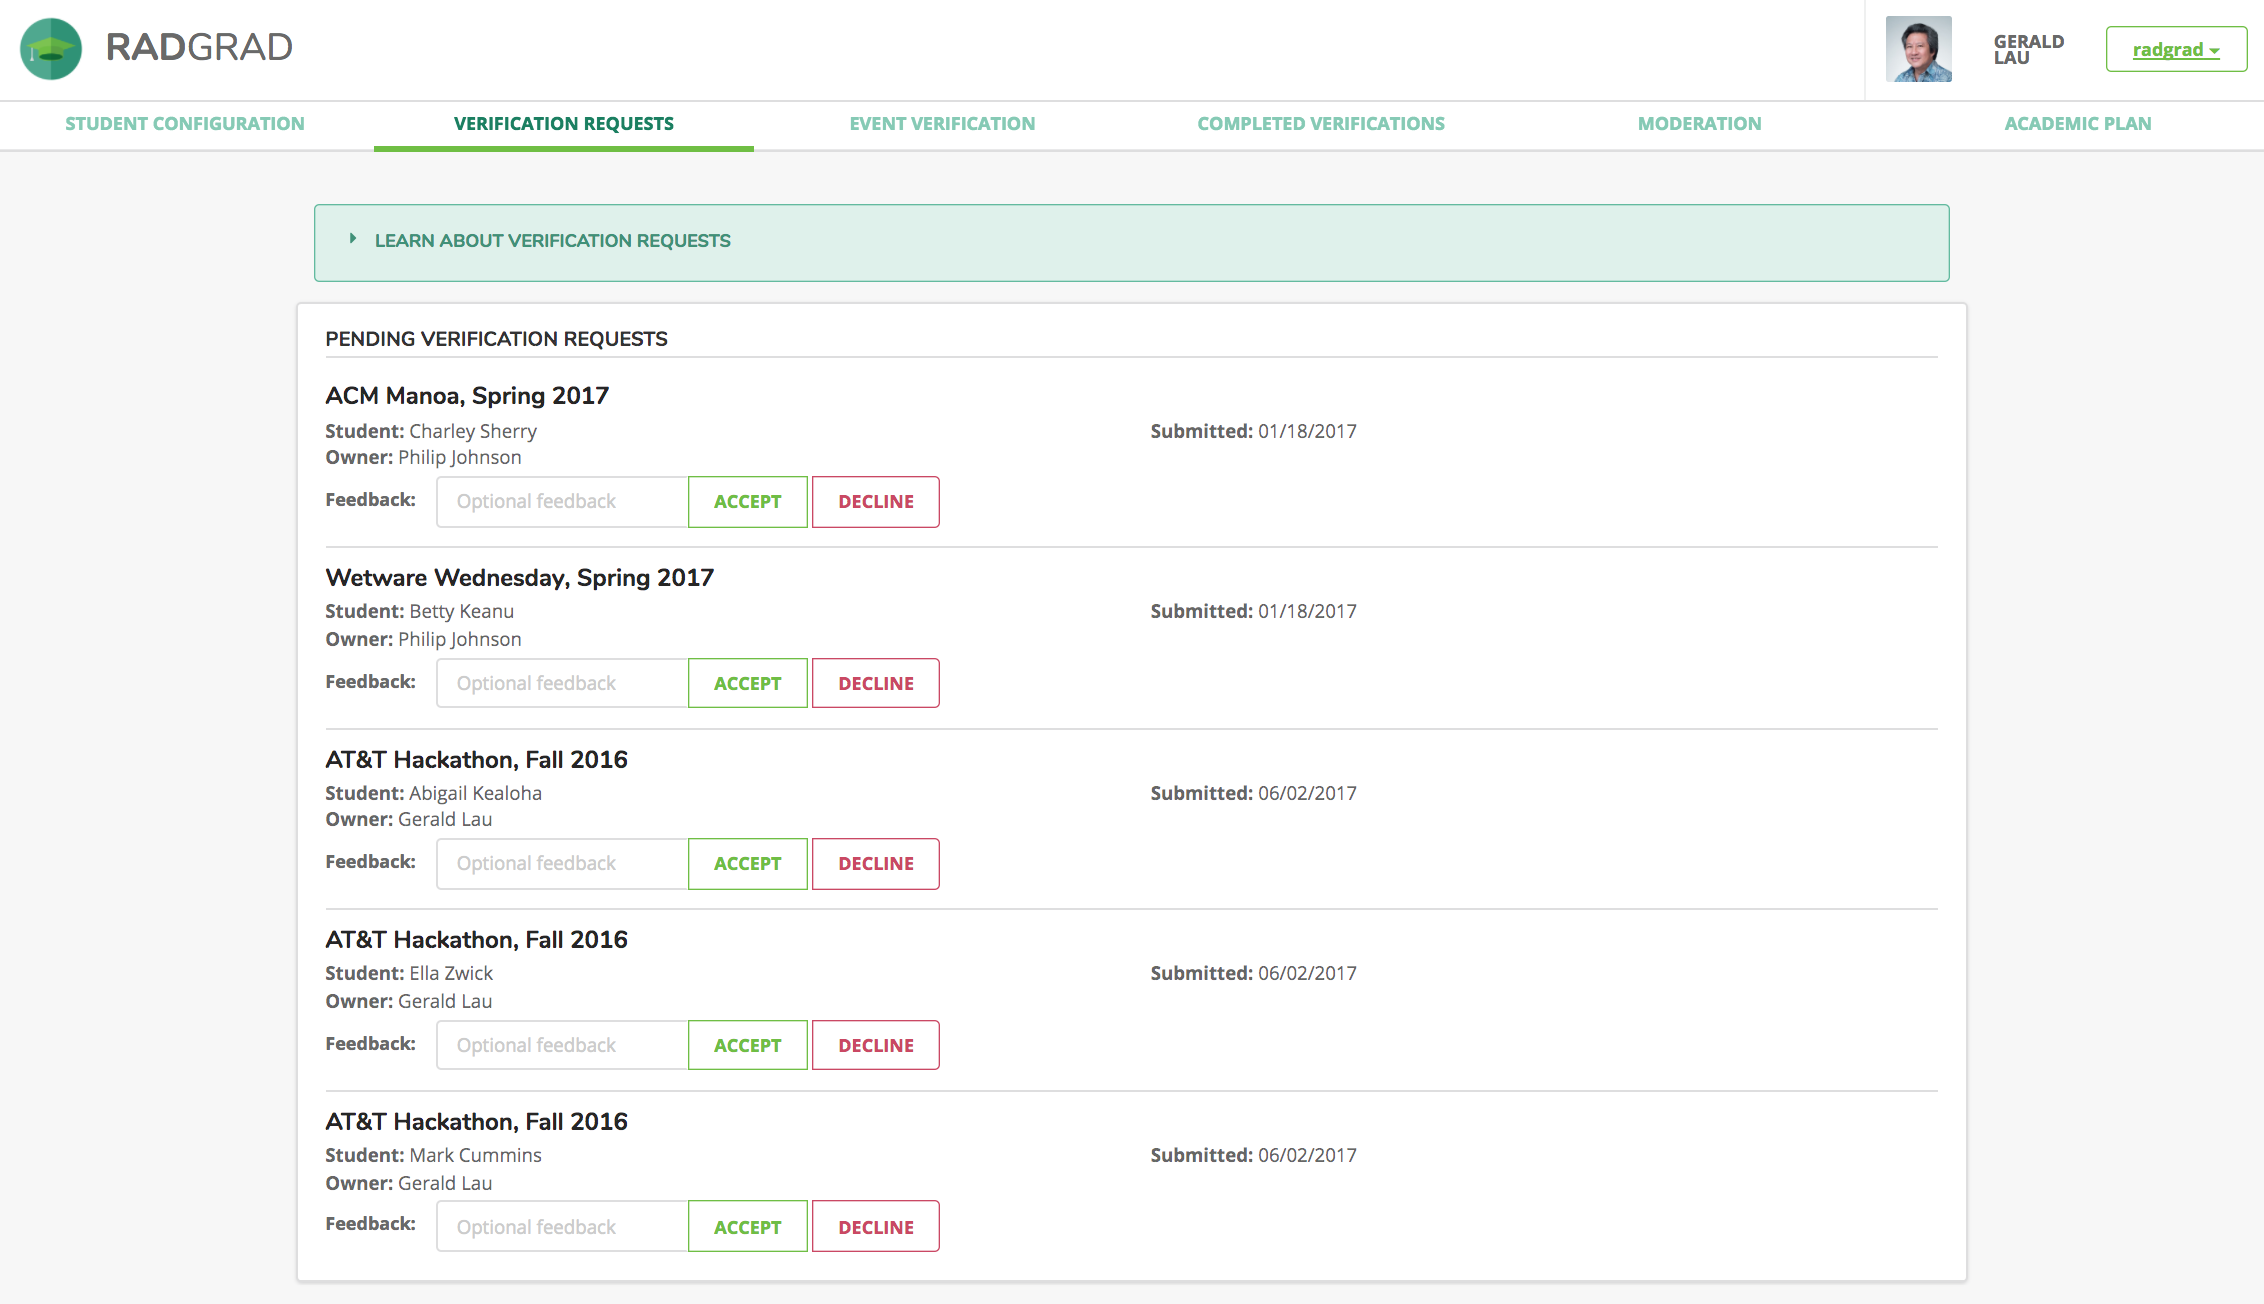
\includegraphics[width=1.0\textwidth]{advisor-verifications}
\caption{Advisor pending verifications page.}
\end{figure}

\begin{figure}[htbp!]
\centering
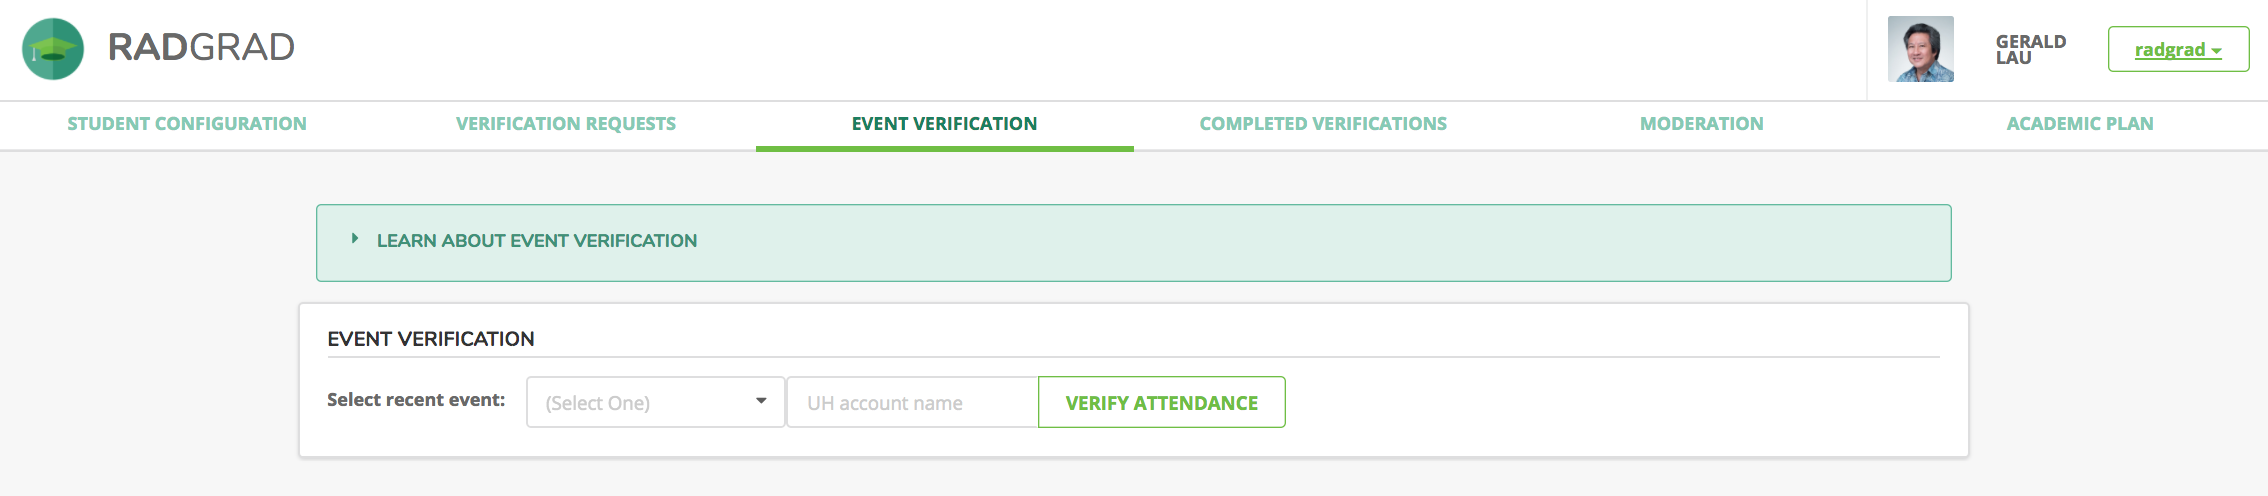
\includegraphics[width=1.0\textwidth]{advisor-eventverification}
\caption{Advisor event verifications page.}
\end{figure}

\begin{figure}[htbp!]
\centering
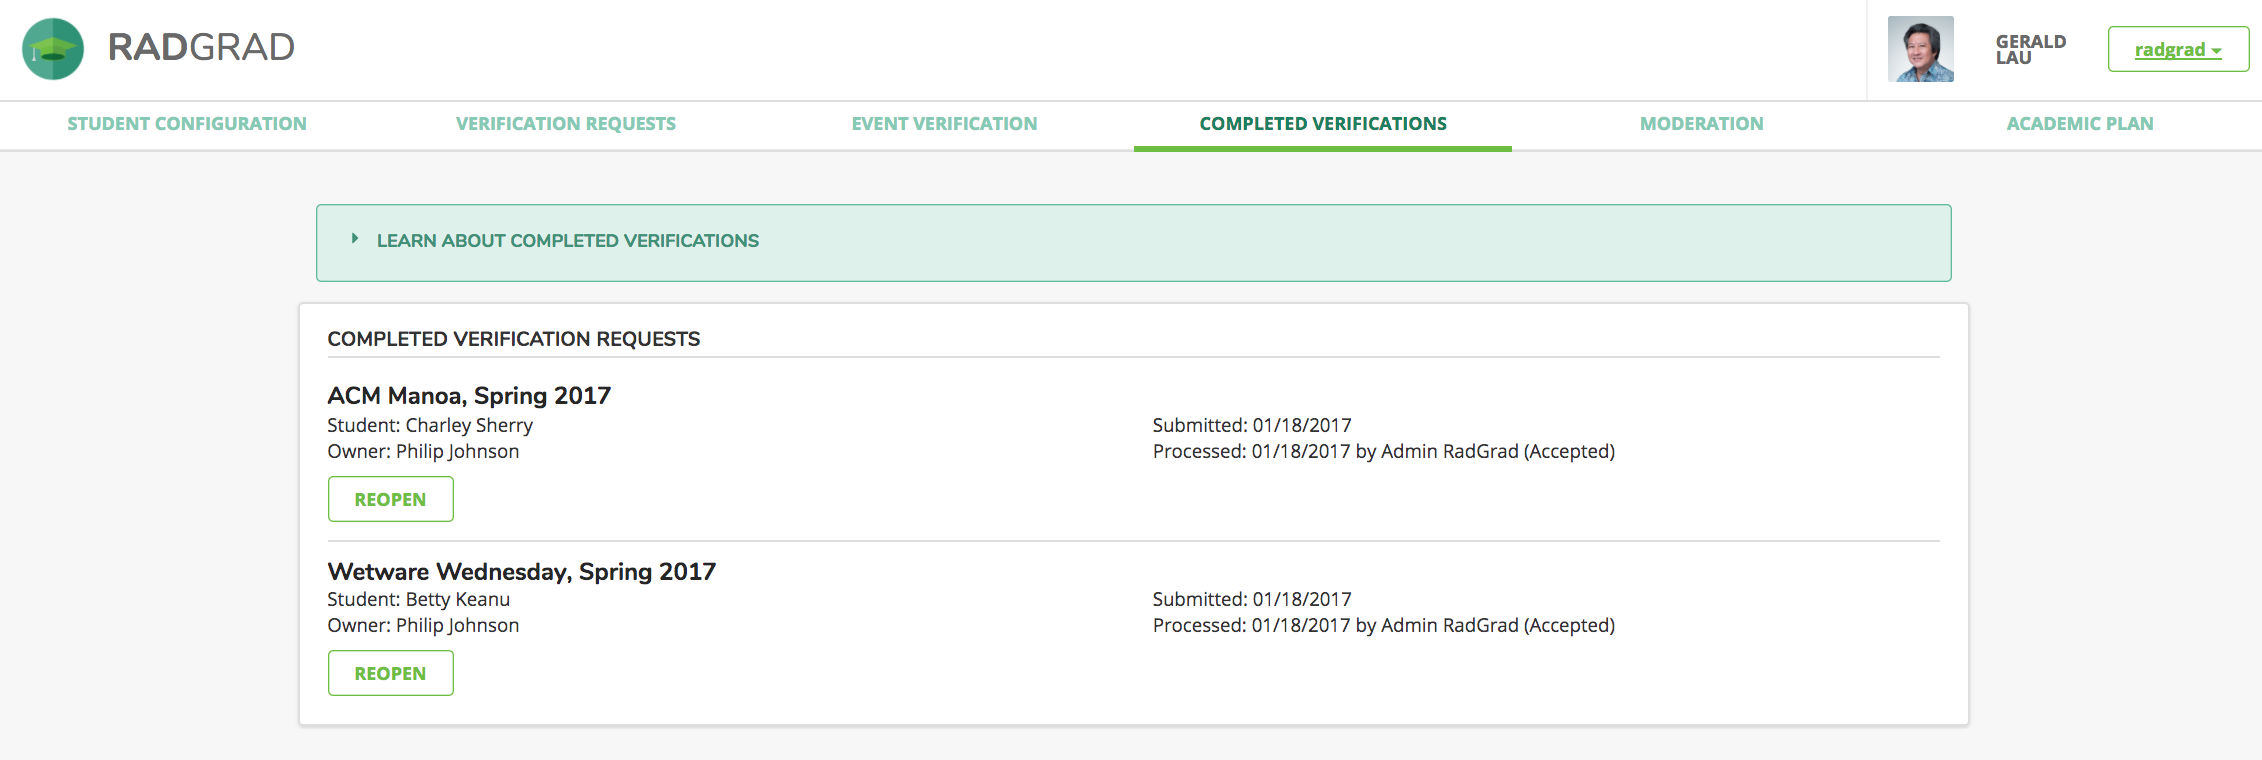
\includegraphics[width=1.0\textwidth]{advisor-completedverifications}
\caption{Advisor completed verifications page.}
\end{figure}
Advisors can verify a student's completion of an opportunity in two ways: with a pending verification (Figure 6.42), and with an event verification (Figure 6.43). If an advisor is physically at an event, and needs to quickly verify a large amount of students, he can use the event verification. In this interface, the advisor simply chooses the event from a dropdown selection of recent events, and then types in the student's UH account name and clicks ``Verify Attendance." If an advisor is not physically present, a student can send a verification request through RadGrad. These requests show up as pending verifications. Advisors can choose to accept or decline these verifications. If they decide to decline, they can leave feedback for the student, and the student can resubmit as many times as they choose. Adivsors can view completed verifications (Figure 6.44) to either simply check past verifications or to reopen a verification.
\subsection{Moderation}
\begin{figure}[htbp!]
\centering
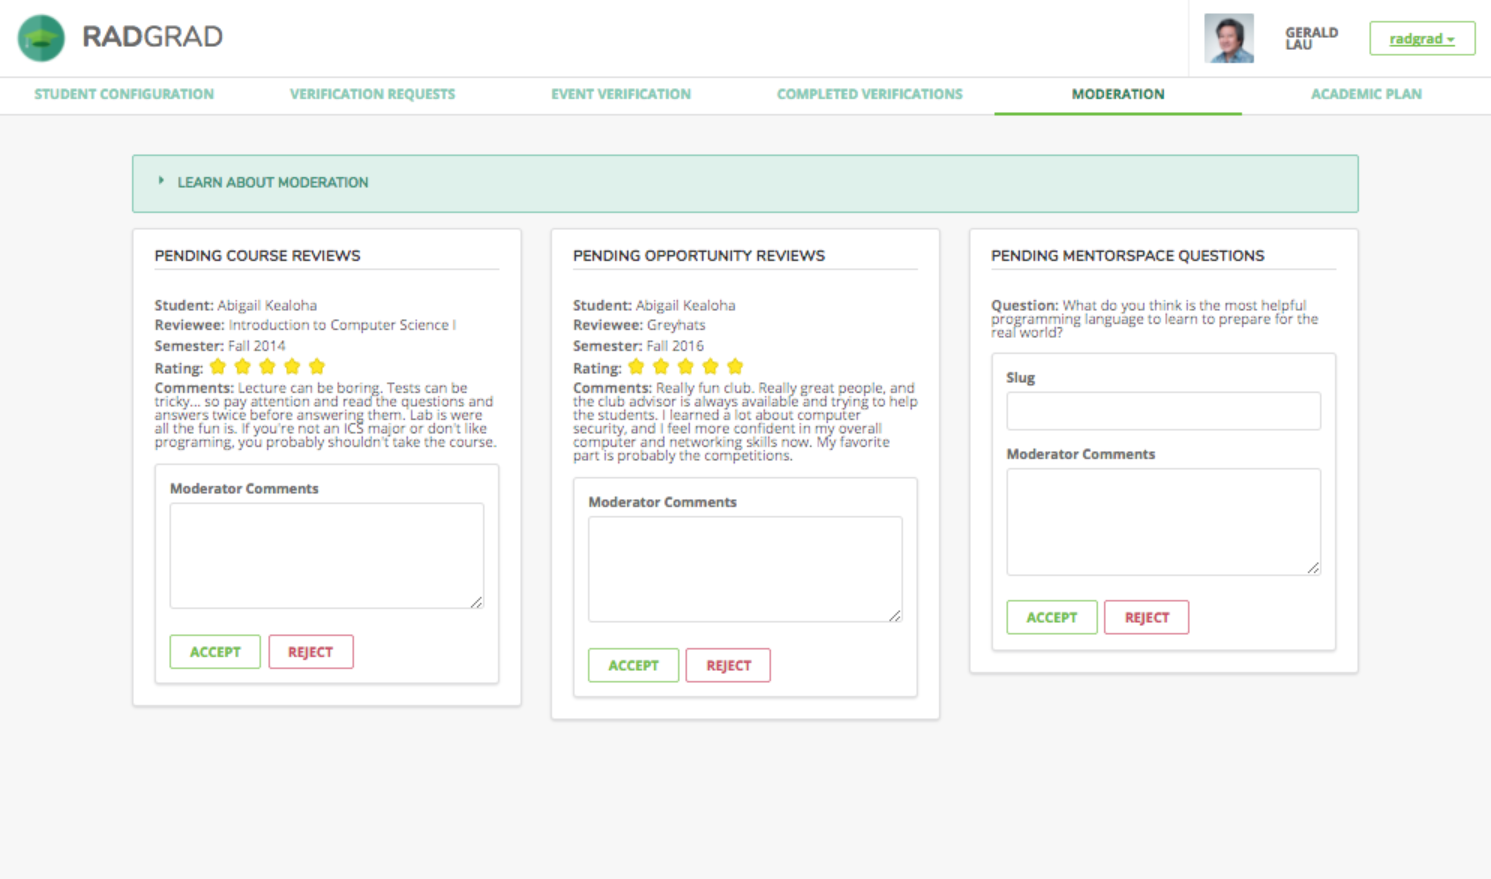
\includegraphics[width=1.0\textwidth]{advisor-moderation}
\caption{Advisor moderation page.}
\end{figure}
Advisors can use the moderation page to moderate course reviews, opportunity reviews, and MentorSpace questions (Figure 6.45). Advisors can choose to either accept or deny these posts. In the case of denial, advisors can leave reasons for denial so that the student can edit and resubmit their post accordingly. 
\subsection{Academic Plan}
\begin{figure}[htbp!]
\centering
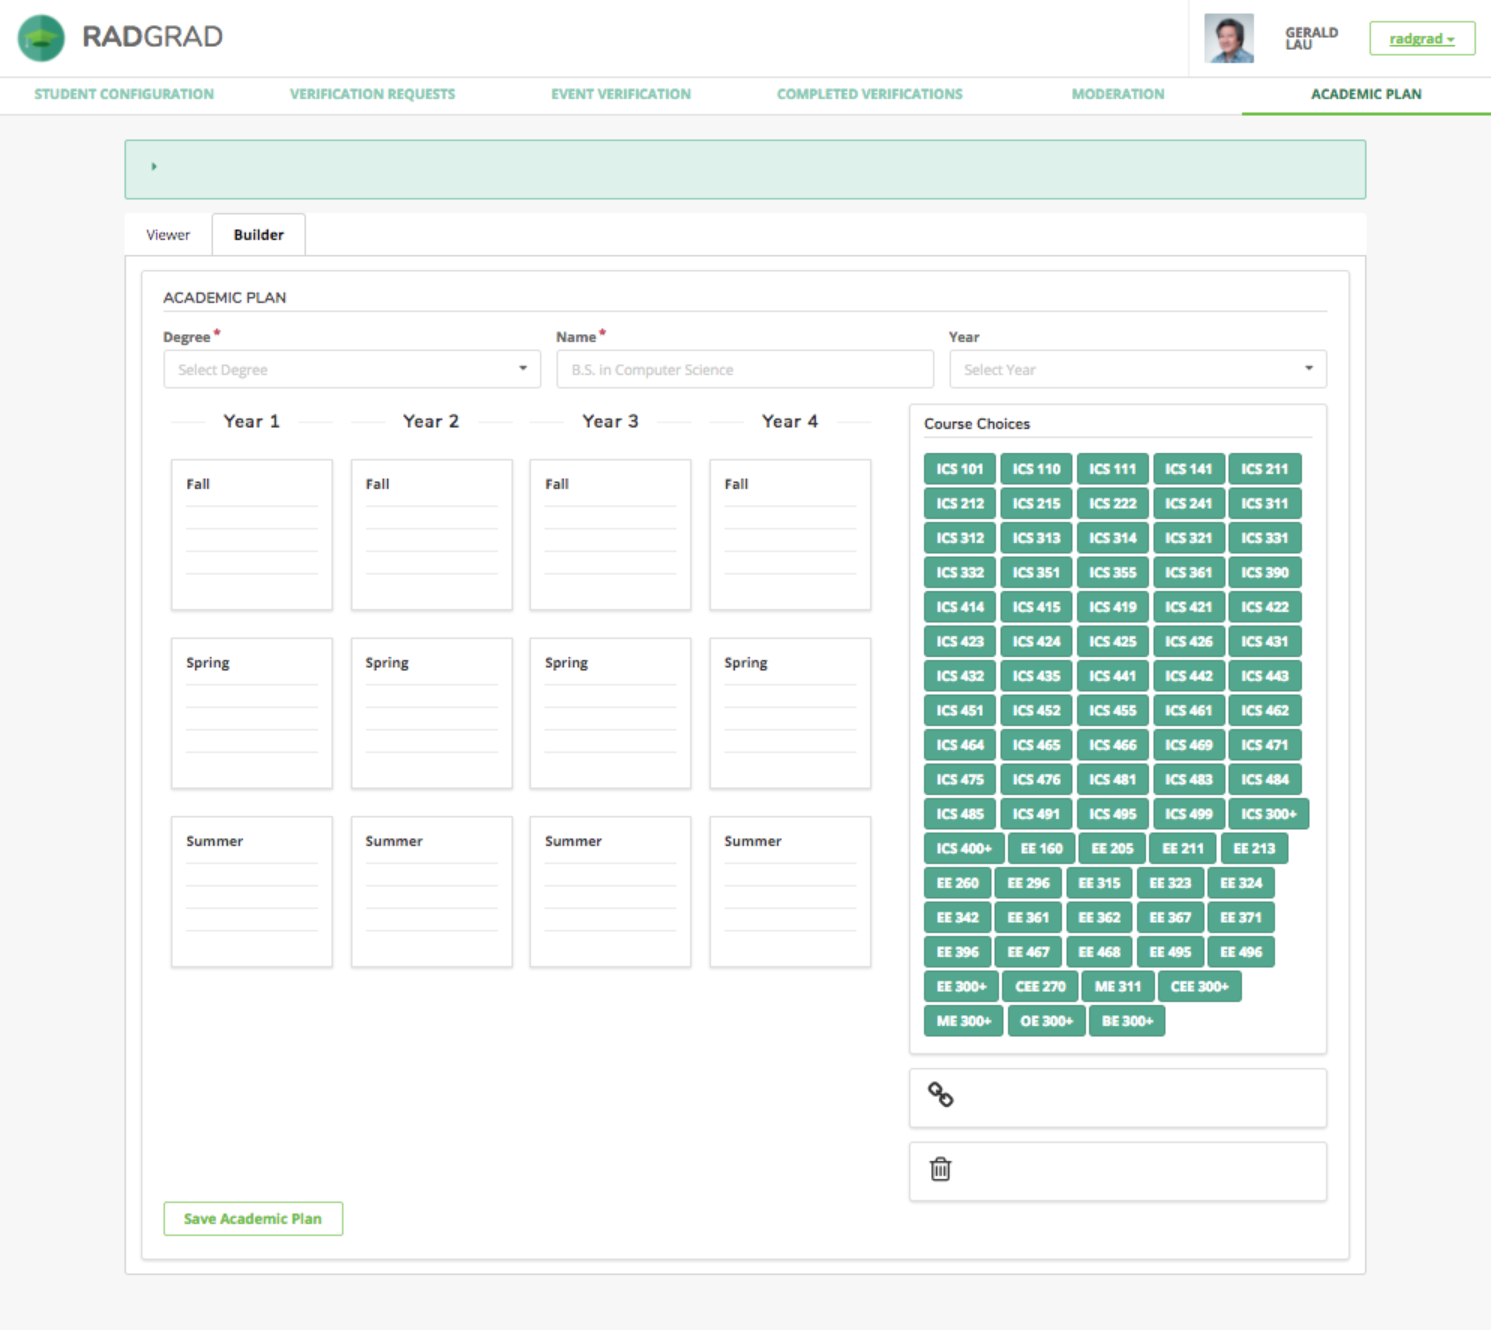
\includegraphics[width=1.0\textwidth]{advisor-academic-plan}
\caption{Advisor academic plan page.}
\end{figure}
The academic plan page is the only place on RadGrad that allows the user to build academic plans (Figure 6.46). There are two tabs: Viewer and Builder. The viewer allows the advisor to choose a year and a plan name, and view the four year plan for that plan. To make any edits to an existing plan or add a new plan, advisors can go over to the builder, which allows them to name a new academic plan with a degree, name, and year. The advisor can then build the four year plan easily by dragging and dropping possible courses onto the initially empty plan. Some plans have more complex requirements than a single courses (i.e. a student must take one course from one of the four groups: ICS312 or ICS331, ICS 313 or ICS361, ICS351 or ICS451, or ICS355). For requirements like this, advisors can easily create groupings by dragging courses to the box with the link icon. Once a complex requirement is completely built, it can be dragged directly onto the plan. If an advisor no longer needs a certain requirement, they can delete it by dragging it to the trash can icon. 

\section{Faculty Mode}
\subsection{Profile}
\begin{figure}[htbp!]
\centering
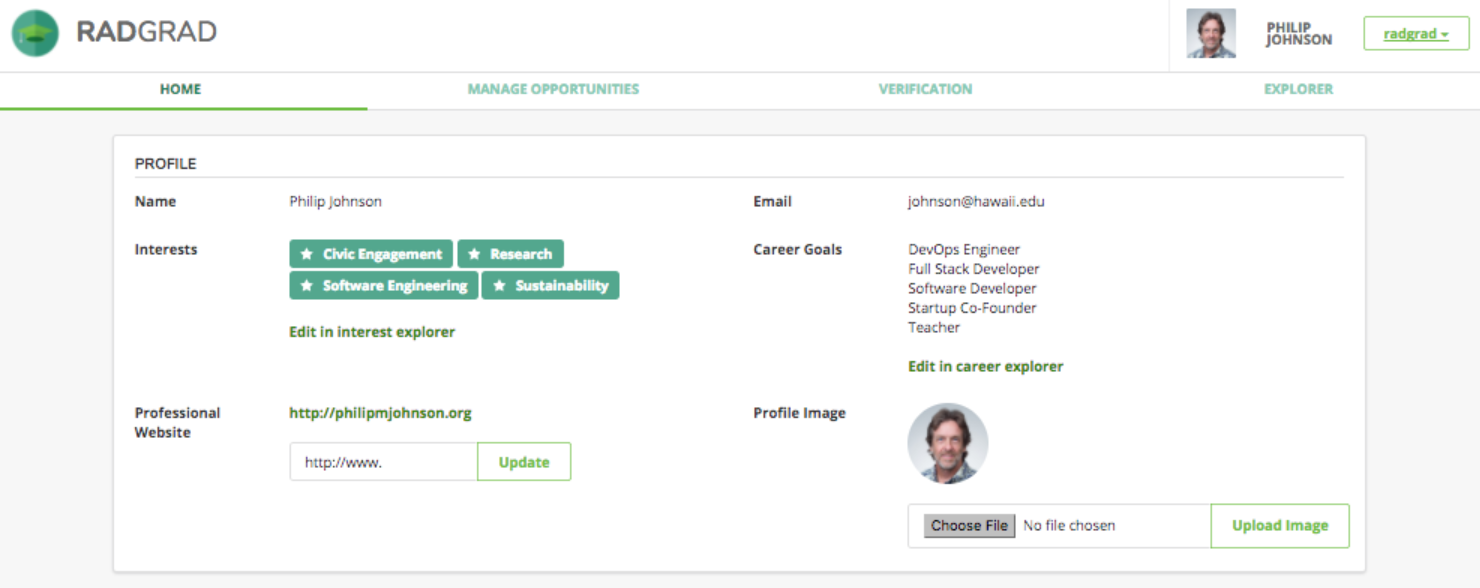
\includegraphics[width=1.0\textwidth]{faculty-profile}
\caption{Faculty profile page.}
\end{figure}
Faculty can use the profile page to view and edit their profile, which reflects how others will see them on RadGrad (Figure 6.47). On this page, faculty can update their photo and information about their website. Faculty can personalize their profiles in a way that accurately communicates their background and research to students. 
\subsection{Manage Opportunities}
\begin{figure}[htbp!]
\centering
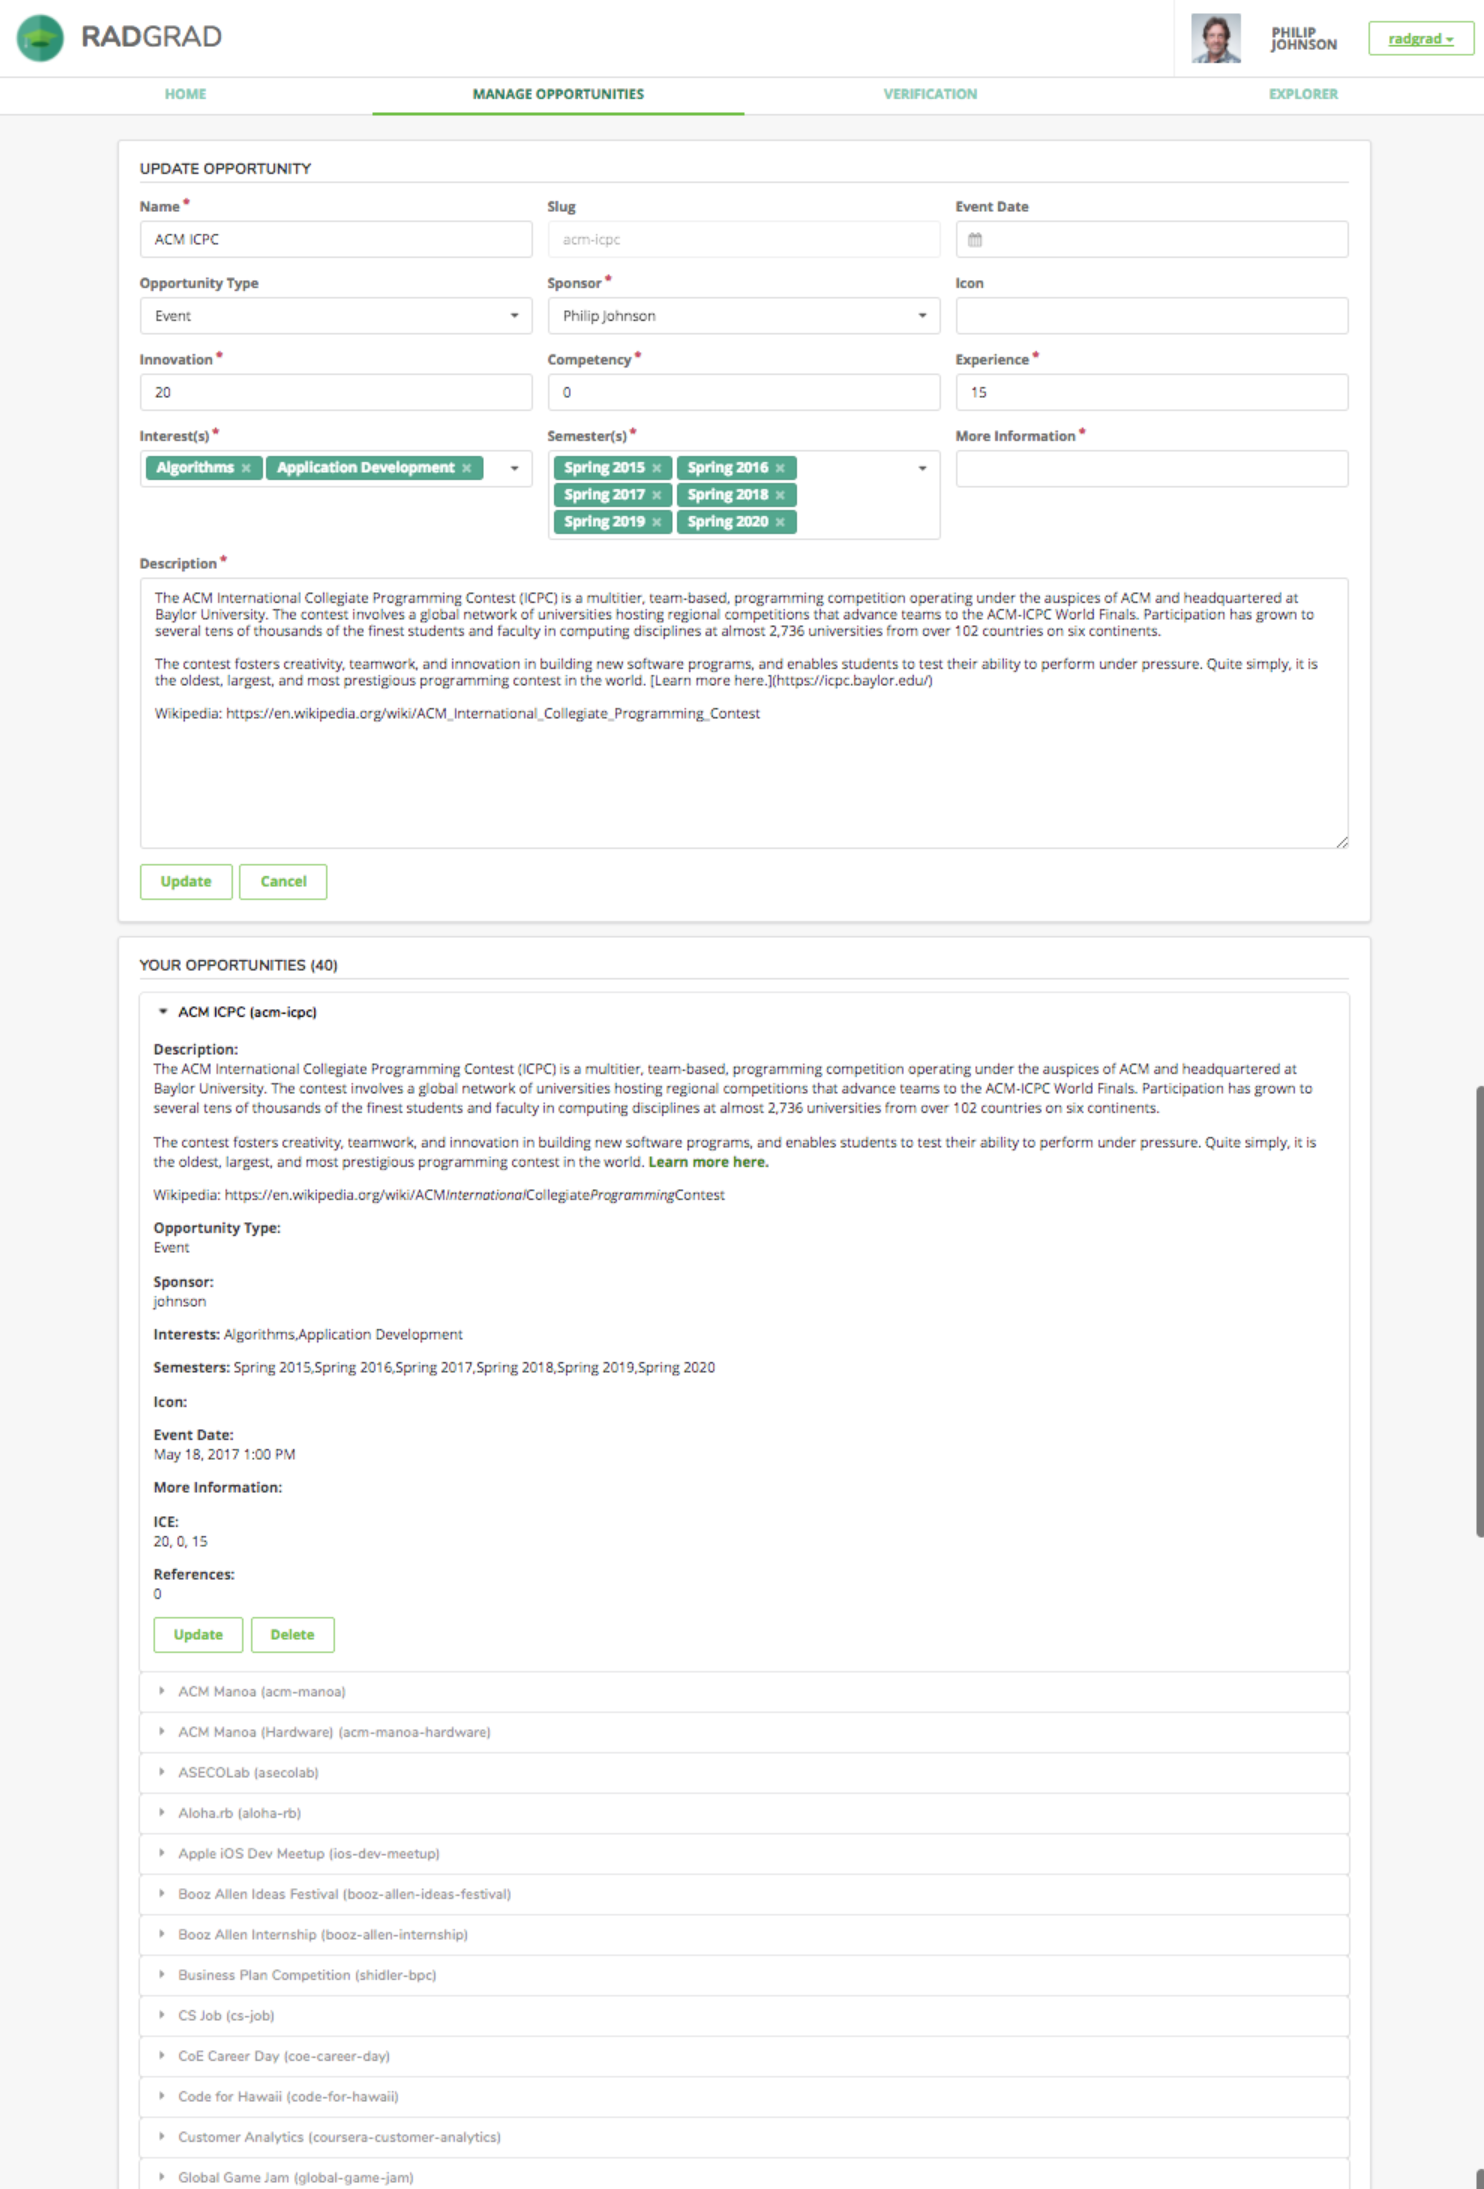
\includegraphics[width=1.0\textwidth]{faculty-opportunity}
\caption{Faculty Manage Opportunities page.}
\end{figure}
Faculty can use the manage opportunities page to easily view, add, edit, or delete their sponsored opportunities (Figure 6.48). They can also view other opportunities, but they can only edit their own. Faculty can edit their opportunities at any time.
\subsection{Verification}
Faculty have the same verification interface as advisors, except they can only view their own verifications for their own sponsored opportunities. 
\subsection{Explorers}
Faculty view the same explorer as students, except they cannot add courses or opportunities, and they cannot leave any type of review. However, they can use the explorer to add interests and career goals. Also, the opportunity explorer conveniently shows the faculty's sponsored opportunities at the top of their opportunity list for quick access.

\section{Mentor Mode}
\subsubsection{Profile}
\begin{figure}[htbp!]
\centering
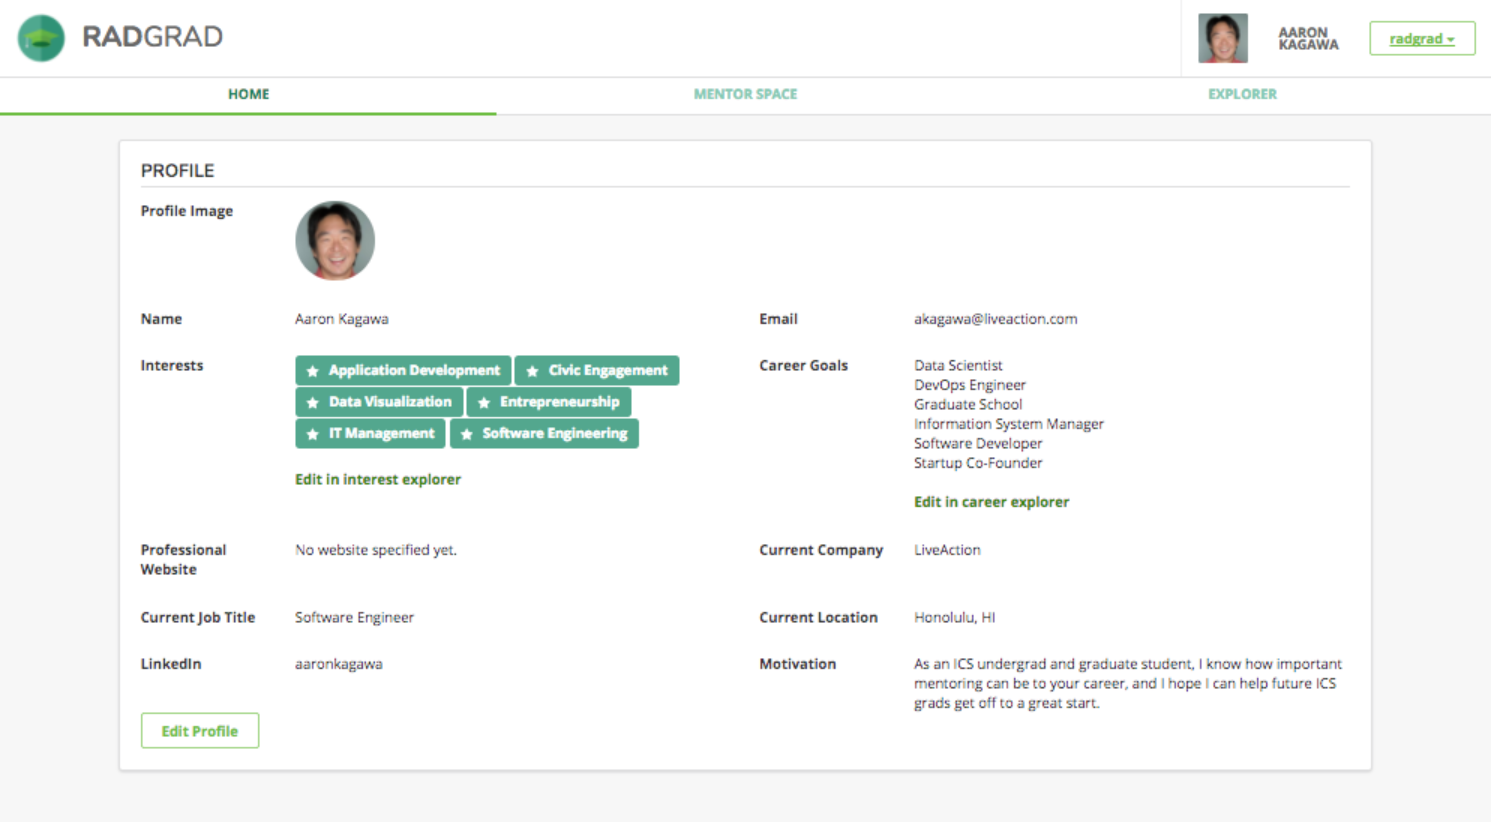
\includegraphics[width=1.0\textwidth]{mentor-profile}
\caption{Mentor profile page.}
\end{figure}
Mentors can use the profile page to view and edit their profile, which reflects how others will see them on RadGrad (Figure 6.49). On this page, mentors can update their photo and information about their website, company, job title, location, LinkedIn, and motivation for becoming a mentor. Mentors can personalize their profiles in a way that accurately communicates their background and willingness to help to the students. 
\subsubsection{MentorSpace}
\begin{figure}[htbp!]
\centering
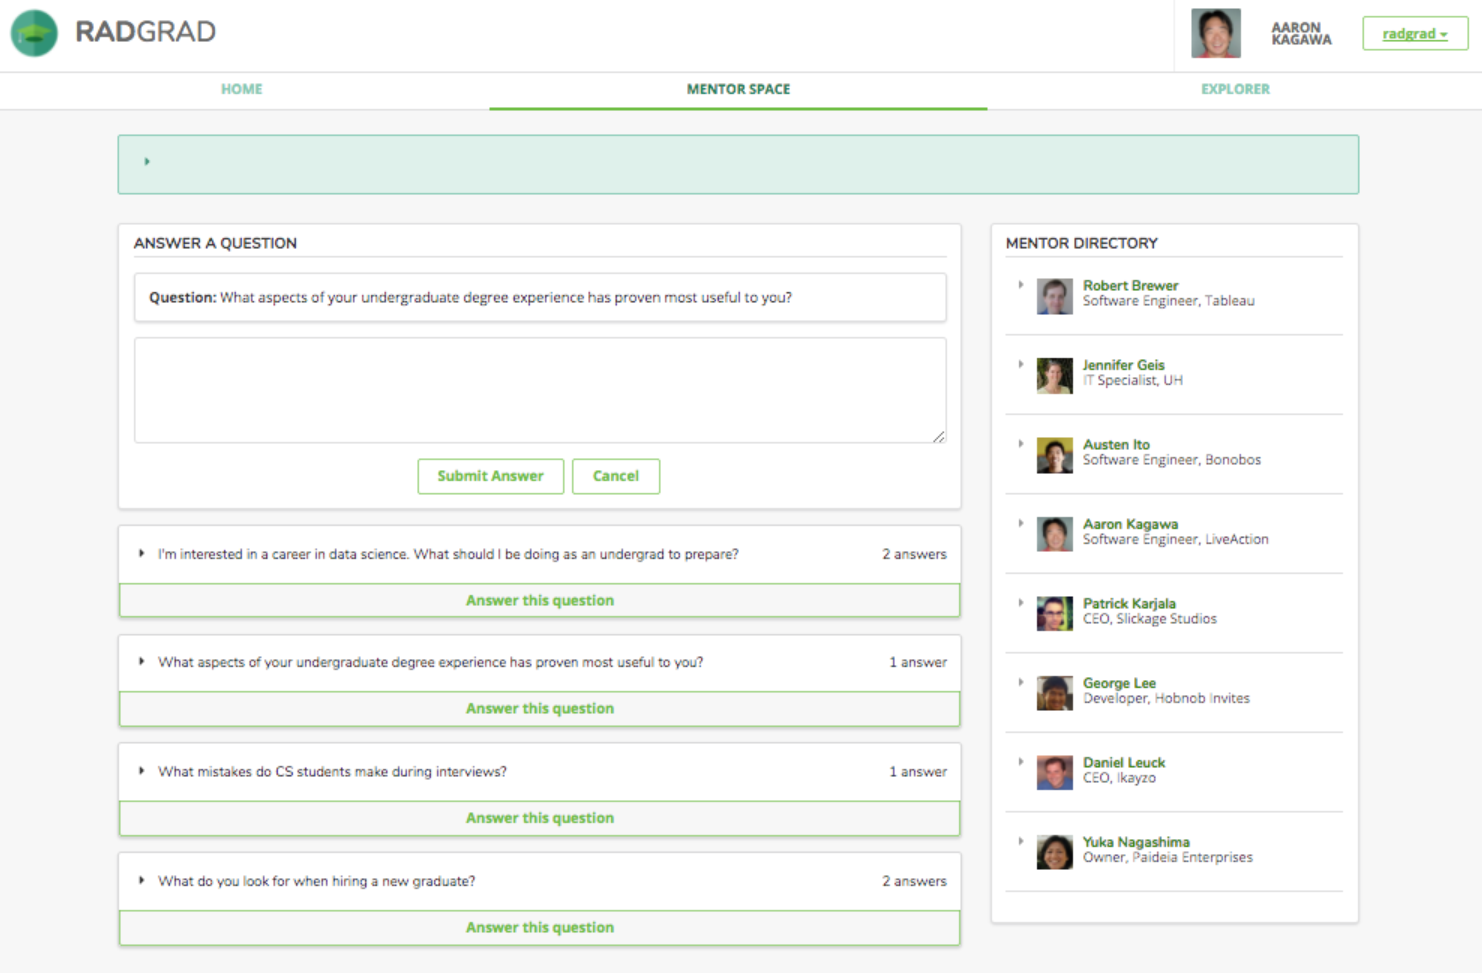
\includegraphics[width=1.0\textwidth]{mentor-mentorspace}
\caption{Mentor MentorSpace Page.}
\end{figure}
Mentors view the same MentorSpace that students do, except each question has an ``Answer this question" or ``Edit your answer" button (Figure 6.5). Clicking on this button brings up a form at the top of the page, which mentors can use to either submit a new answer or revise their existing answer. 
\subsubsection{Explorer}
Mentors view the same explorer as students, except they cannot add courses or opportunities, and they cannot leave any type of review. However, they can use the explorer to add interests and career goals.

\section{Administrator Mode}
\subsection{Retrieve User}
\begin{figure}[htbp!]
\centering
\includegraphics[width=1.0\textwidth]{admin-retrieve-user}
\caption{Administrator Retrieve User page.}
\end{figure}
On the Administrator home page, an administrator can access any user's account (Figure 6.51). Users are organized by role (on tabs) and then alphabetically by last name. Clicking on the user's name will lead to their profile. Administrators can use this for testing or troubleshooting purposes. On the student tab, there is also a button to update student levels. Clicking this button will automatically recalculate and set the levels for all of the students.

\subsection{Data Model}
\begin{figure}[htbp!]
\centering
\includegraphics[width=1.0\textwidth]{admin-datamodel}
\caption{Administrator Data Model page.}
\end{figure}
The data model page allows administrators to view, add, edit, and delete items from the data model (Figure 6.52). The menu on the left lists all collections. When an administrator clicks on a collection, they will see a form, which they can use manipulate items in that collection. Below the form, they can view a list of all existing collection items. 
\subsection{Data Base}
\begin{figure}[htbp!]
\centering
\includegraphics[width=1.0\textwidth]{admin-database}
\caption{Administrator Data Base page.}
\end{figure}
The database page allows administrators to easily run an integrity check on the database, dump the database, and restore the database (Figure 6.53)
. The integrity check tests every item in the database to make sure that all parts of it are valid. Dumping the database saves the current state of the database to a JSON file and downloads it to your computer. Restoring the database deletes the current database and reloads an earlier version from a JSON file. Administrators can use this in backup and testing situations.
\subsection{Moderation}
Administrators have the same moderation page as advisors. 